\chapter{HASIL DAN PEMBAHASAN}


\section{Hasil Perancangan dan Pengembangan}
Bagian ini memaparkan hasil implementasi dari rancangan sistem yang telah didefinisikan pada bab sebelumnya. Pemaparan hasil pengembangan mencakup realisasi arsitektur sistem agentik yang menjadi kerangka kerja utama, konfigurasi agen LLM beserta instruksi sistem yang mengatur perilakunya, serta integrasi modul-modul pendukung kecerdasan sistem seperti deteksi objek dan pengambilan informasi. Selain aspek fungsionalitas inti, hasil pengembangan antarmuka pengguna juga disajikan untuk menunjukkan wujud interaksi antara pengguna dengan sistem yang telah dibangun.

\subsection{Sistem Agentik}
Implementasi sistem agentik telah berhasil direalisasikan menggunakan kerangka kerja LangChain dan pustaka LangGraph sesuai dengan rancangan yang telah dibahas sebelumnya. Sistem ini memodelkan perilaku agen LLM dalam struktur graf berstatus untuk menangani tugas identifikasi penyakit tanaman secara adaptif. Ketika definisi dari graf agen dikompilikasi, dihasilkan keluaran berupa visualisai graf pada Gambar \ref{fig:compiled_state_graph}. Representasi ini menunjukkan struktur topologi graf yang terbentuk setelah kode program dieksekusi. Simpul-simpul utama yang merepresentasikan logika pengambilan keputusan agen dan eksekusi tindakan alat telah terbentuk dan terhubung oleh sisi-sisi yang mengatur aliran kontrol. Struktur ini memvalidasi bahwa desain pola ReAct telah berhasil diterjemahkan ke dalam objek eksekutif yang siap dijalankan.

\begin{figure}[H]
    \centering
    
\includegraphics[width=0.4\textwidth]{bab4/compiledstategraph.png}
    \caption[Representasi graf sistem agentik]{Representasi graf sistem agentik setelah proses kompilasi}
    \label{fig:compiled_state_graph}
\end{figure}

Verifikasi lebih lanjut terhadap struktur dan alur kerja agen dilakukan menggunakan platform LangSmith. Gambar \ref{fig:agent_graph_langsmith} menampilkan visualisasi graf agen dalam lingkungan LangSmith Studio. Visualisasi ini memberikan gambaran yang lebih interaktif mengenai bagaimana agen berpindah dari satu status ke status lainnya, mulai dari inisialisasi, evaluasi model, pemanggilan alat, hingga terminasi proses. Kesesuaian antara graf yang dirancang dan visualisasi ini mengonfirmasi integritas implementasi alur kerja sistem.

\begin{figure}[H]
    \centering
    
\includegraphics[width=1\textwidth]{bab4/agentgraphdilangsmithstudio.png}
    \caption[Visualisasi graf agen]{Visualisasi graf agen pada LangSmith Studio}
    \label{fig:agent_graph_langsmith}
\end{figure}

\subsection{Agen LLM}
Perancangan dan pengembangan agen LLM difokuskan pada implementasi \textit{prompt} sistem (\textit{system prompt}) dan konfigurasi model untuk memastikan perilaku agen sesuai dengan parameter yang telah dirancang. Implementasi ini mencakup manajemen \textit{prompt} menggunakan LangSmith Prompt Hub serta realisasi kerangka kerja CO-STAR. Manajemen instruksi dilakukan secara terpusat menggunakan layanan LangSmith Prompt Hub. Pendekatan ini memisahkan logika kode program dengan konfigurasi instruksi bahasa alami, yang memungkinkan proses iterasi dan pembaruan instruksi dilakukan tanpa mengubah kode sumber aplikasi secara langsung. Gambar \ref{fig:langsmith_prompt_hub} menampilkan antarmuka manajemen \textit{prompt} yang digunakan, di mana versi \textit{prompt} dikelola dan dilacak perubahannya.

\begin{figure}[H]
    \centering
    
\includegraphics[width=1\textwidth]{bab4/tampilanpromptdilangsmithprompthub.png}
    \caption[Tampilan antarmuka manajemen \textit{prompt}]{Tampilan antarmuka manajemen \textit{prompt} pada LangSmith Prompt Hub}
    \label{fig:langsmith_prompt_hub}
\end{figure}

Kerangka kerja CO-STAR yang dirancang pada tahap sebelumnya telah diterjemahkan menjadi bagian-bagian instruksi terstruktur. Bagian \textit{context} menetapkan peran agen sebagai ahli patologi tanaman dengan batasan domain yang ketat, sedangkan bagian \textit{objective} menekankan pada jawaban yang berbasis bukti (\textit{evidence-grounded}). Cuplikan implementasi instruksi bagian \textit{context} dan \textit{objective} disajikan dalam Gambar \ref{fig:prompt_context}.

\begin{figure}[H]
    \centering
    
\includegraphics[width=1\textwidth]{bab4/contextobjective.png}
    \caption[Realisasi instruksi \textit{context} dan \textit{objective}]{Realisasi instruksi \textit{context} dan \textit{objective} pada sistem}
    \label{fig:prompt_context}
\end{figure}

Selanjutnya, bagian \textit{style}, \textit{tone}, dan \textit{audience} mendefinisikan persona agen dalam berinteraksi. Agen diinstruksikan untuk selalu menyesuaikan bahasa dengan pengguna, membedakan secara tegas antara observasi visual dan inferensi, serta mempertahankan nada yang tenang dan jujur mengenai ketidakpastian. Target audiens yang bervariasi dari pemilik tanaman hingga profesional pertanian menuntut penjelasan yang jelas tanpa jargon berlebih. Implementasi ketiga bagian ini ditampilkan pada Gambar \ref{fig:prompt_sta}.

\begin{figure}[H]
    \centering
    
\includegraphics[width=1\textwidth]{bab4/styletoneaudience.png}
    \caption[Realisasi instruksi \textit{style}, \textit{tone}, dan \textit{audience}]{Realisasi instruksi \textit{style}, \textit{tone}, dan \textit{audience} pada sistem}
    \label{fig:prompt_sta}
\end{figure}

Terakhir, bagian \textit{response} menetapkan struktur standar untuk jawaban identifikasi yang mewajibkan penggunaan observasi visual, integrasi konteks, hingga identifikasi dengan penalaran. Struktur ini juga mencakup mekanisme tindak lanjut (\textit{follow-up}) jika data kurang mencukupi serta batasan ketat mengenai apa yang tidak boleh disertakan seperti resep kimia atau saran medis. Detail instruksi struktur respons disajikan pada Gambar \ref{fig:prompt_response}.

\begin{figure}[H]
    \centering
    
\includegraphics[width=1\textwidth]{bab4/response.png}
    \caption[Realisasi instruksi \textit{response structure}]{Realisasi instruksi \textit{response structure} pada sistem}
    \label{fig:prompt_response}
\end{figure}


Agar agen dapat berinteraksi dengan alat yang disediakan dengan baik, instruksi sistem juga menyertakan referensi teknis mengenai alat-alat yang tersedia (\textit{tools reference}). Bagian ini memberikan spesifikasi formal untuk fungsi seperti \textit{web\_search} dan \textit{knowledgebase\_search} dalam modul pengambilan informasi, mencakup parameter, tujuan, dan contoh penggunaannya. Referensi ini memastikan agen dapat menyusun pemanggilan alat yang valid secara sintaksis dan semantik. Contoh referensi penggunaan alat tersebut ditampilkan pada Gambar \ref{fig:prompt_tools}.

\begin{figure}[H]
    \centering
    
\includegraphics[width=1\textwidth]{bab4/referensitool.png}
    \caption[Realisasi referensi teknis alat]{Realisasi referensi teknis alat pada sistem}
    \label{fig:prompt_tools}
\end{figure}

Agen juga dilengkapi dengan kebijakan penggunaan alat (\textit{tool decision policy}) yang dirancang untuk mengoptimalkan akurasi dan efisiensi biaya. Kebijakan ini mengatur alur pengambilan keputusan agen mulai dari validasi kualitas citra, pemilihan strategi deteksi, yakni apakah menggunakan deteksi objek atau klasifikasi langsung, hingga mekanisme validasi hasil dan tindakan pemulihan (\textit{fallback}) jika terjadi inkonsistensi. Selain itu, aturan keselamatan (\textit{safety rules}) diterapkan untuk mencegah halusinasi, seperti kewajiban melakukan validasi visual sebelum memanggil alat deteksi dan larangan memberikan saran medis tanpa rujukan. Realisasi kebijakan ini dalam instruksi sistem agen ditampilkan pada Gambar \ref{fig:tool_decision_policy}.

\begin{figure}[H]
    \centering
    \begin{subfigure}[t]{0.48\textwidth}
        \centering
        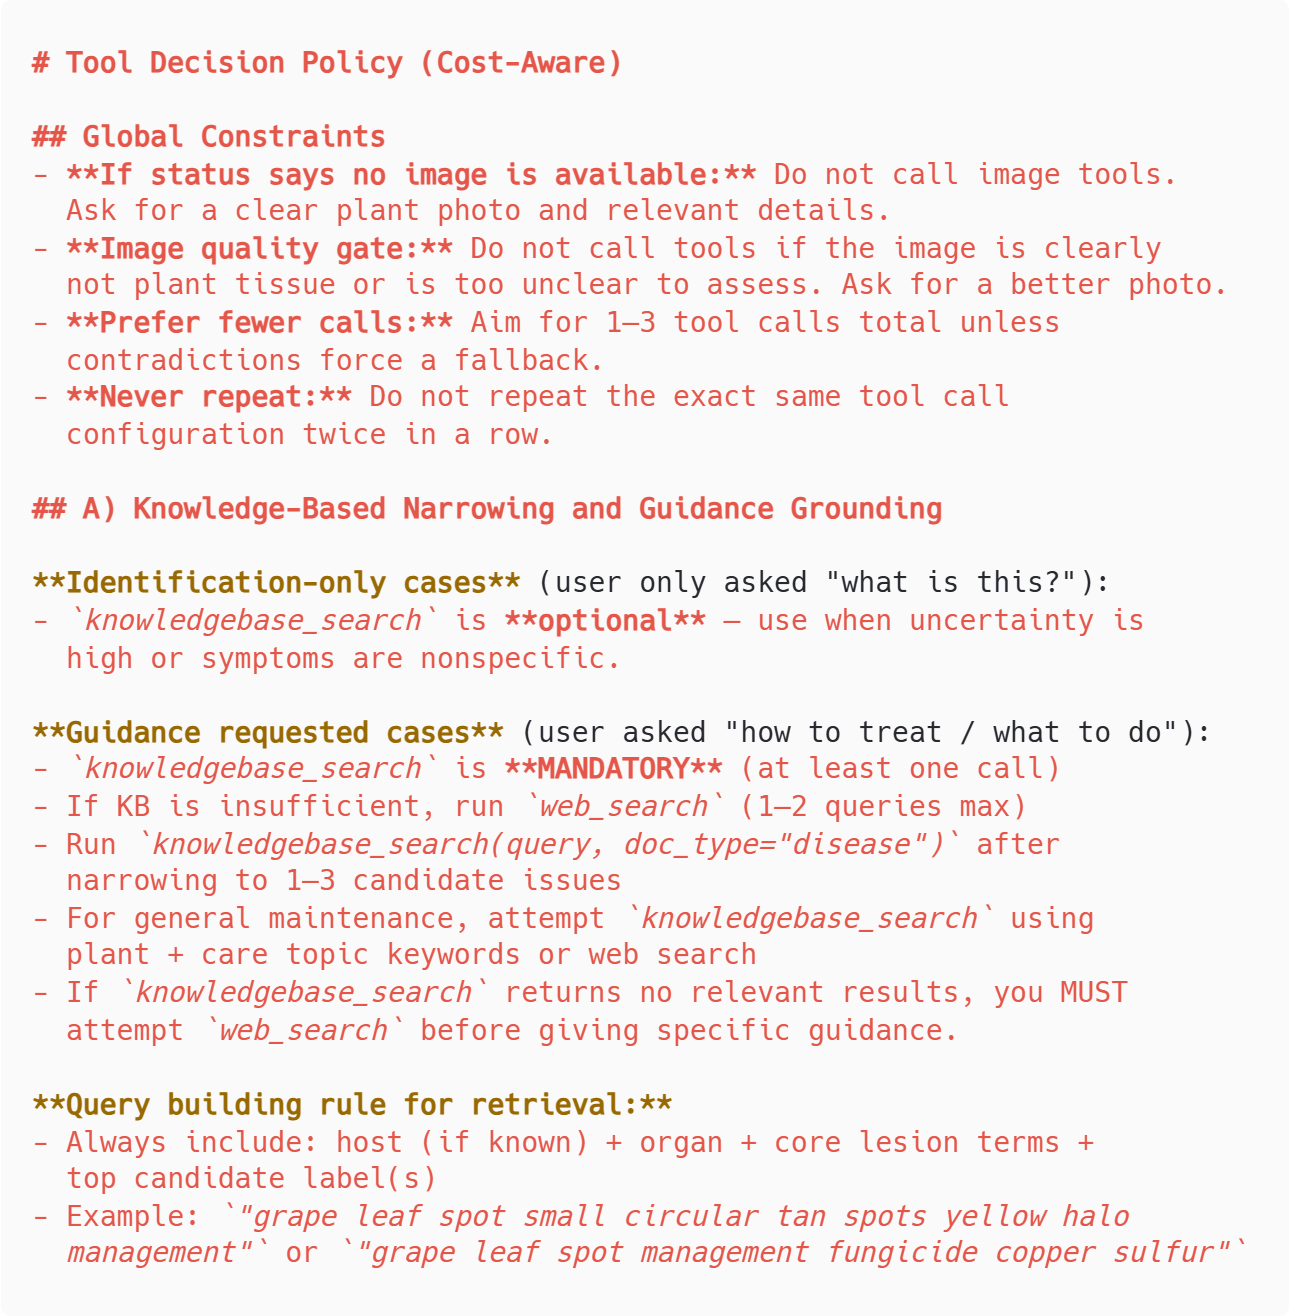
\includegraphics[width=\textwidth]{images/bab4/tool_decision_policy_1.png}
        \caption{}
    \end{subfigure}
    \hfill
    \begin{subfigure}[t]{0.48\textwidth}
        \centering
        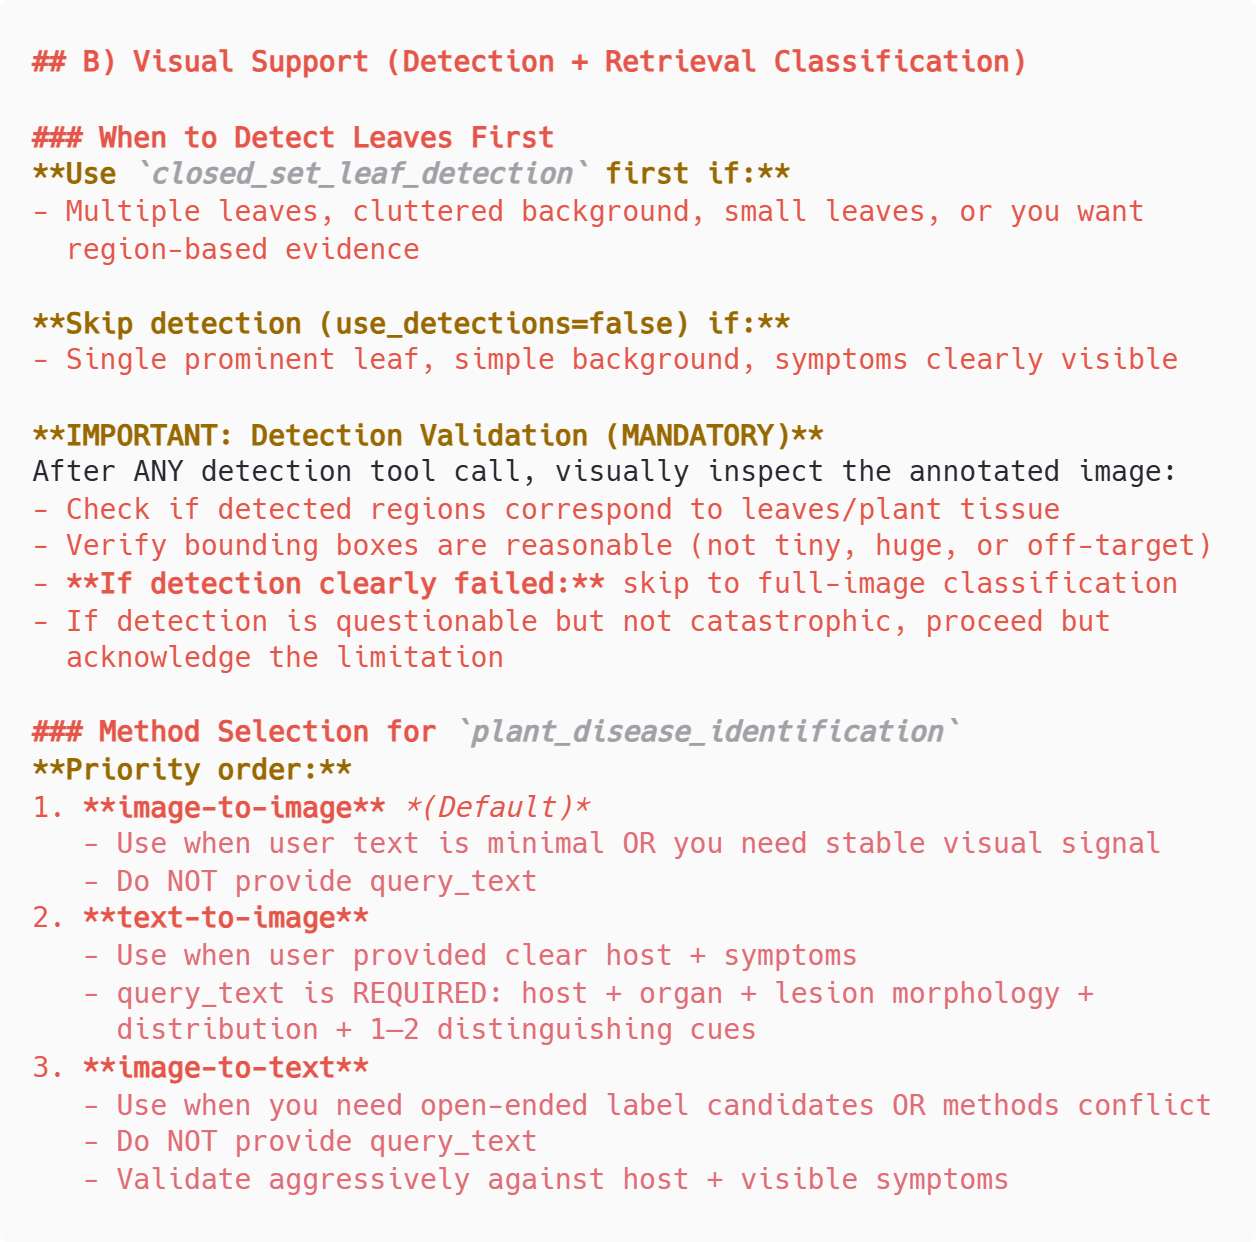
\includegraphics[width=\textwidth]{images/bab4/tool_decision_policy_2.png}
        \caption{}
    \end{subfigure}
    % \vspace{0.5cm}
    \begin{subfigure}[t]{0.48\textwidth}
        \centering
        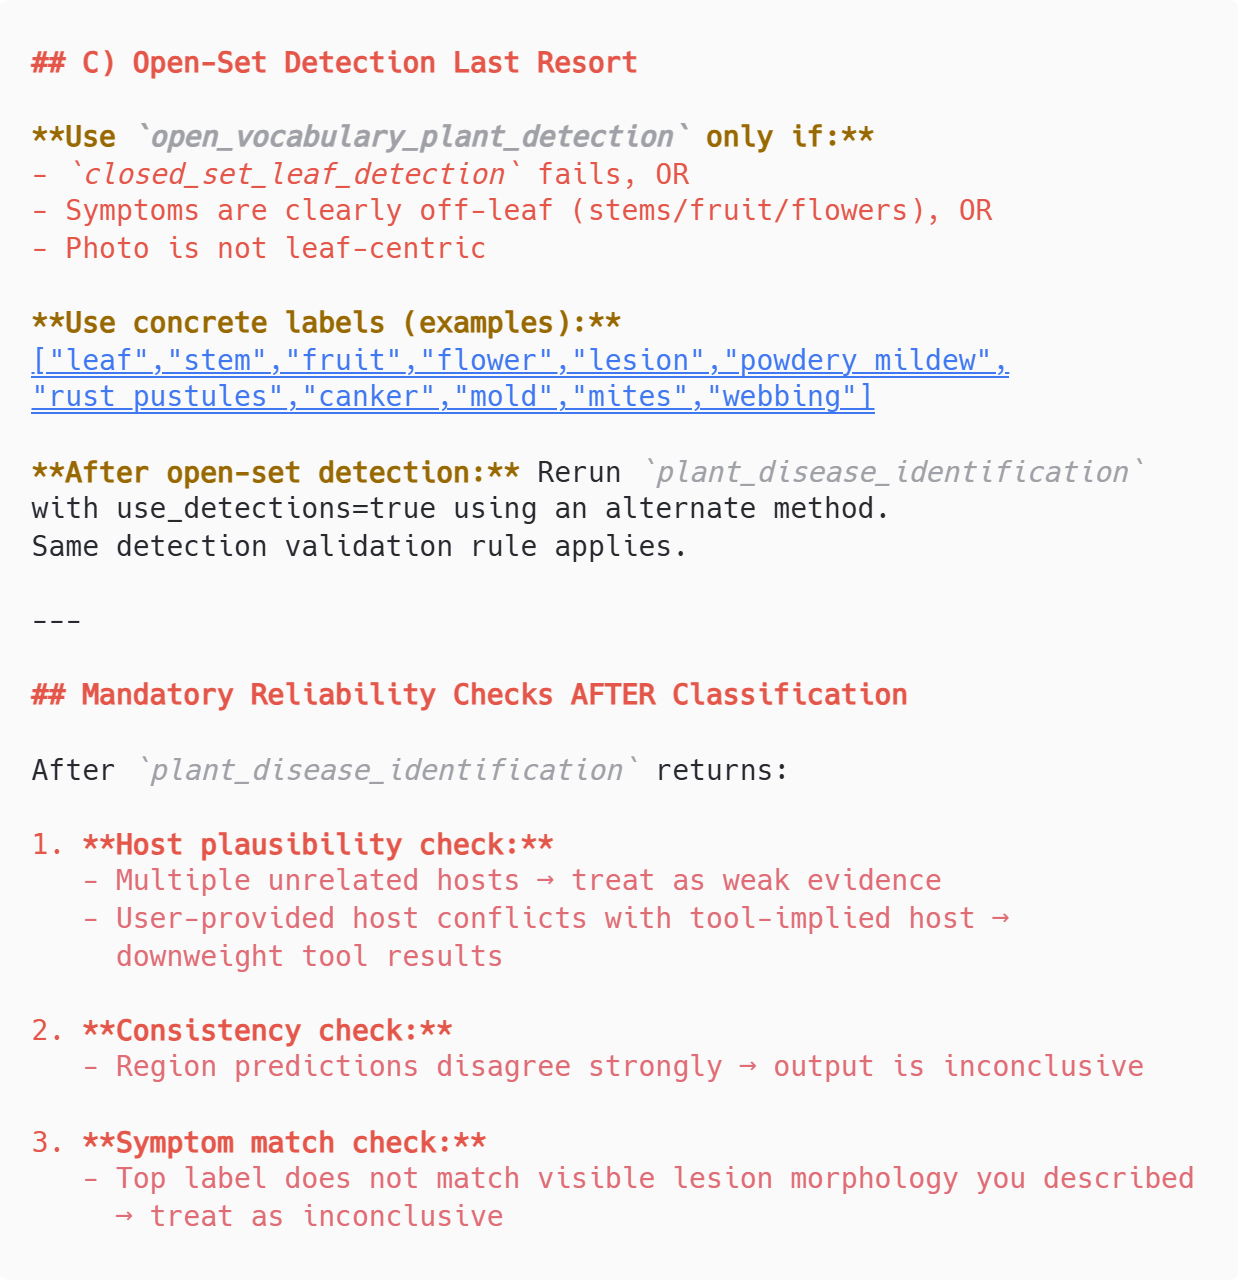
\includegraphics[width=\textwidth]{images/bab4/tool_decision_policy_3.png}
        \caption{}
    \end{subfigure}
    \hfill
    \begin{subfigure}[t]{0.48\textwidth}
        \centering
        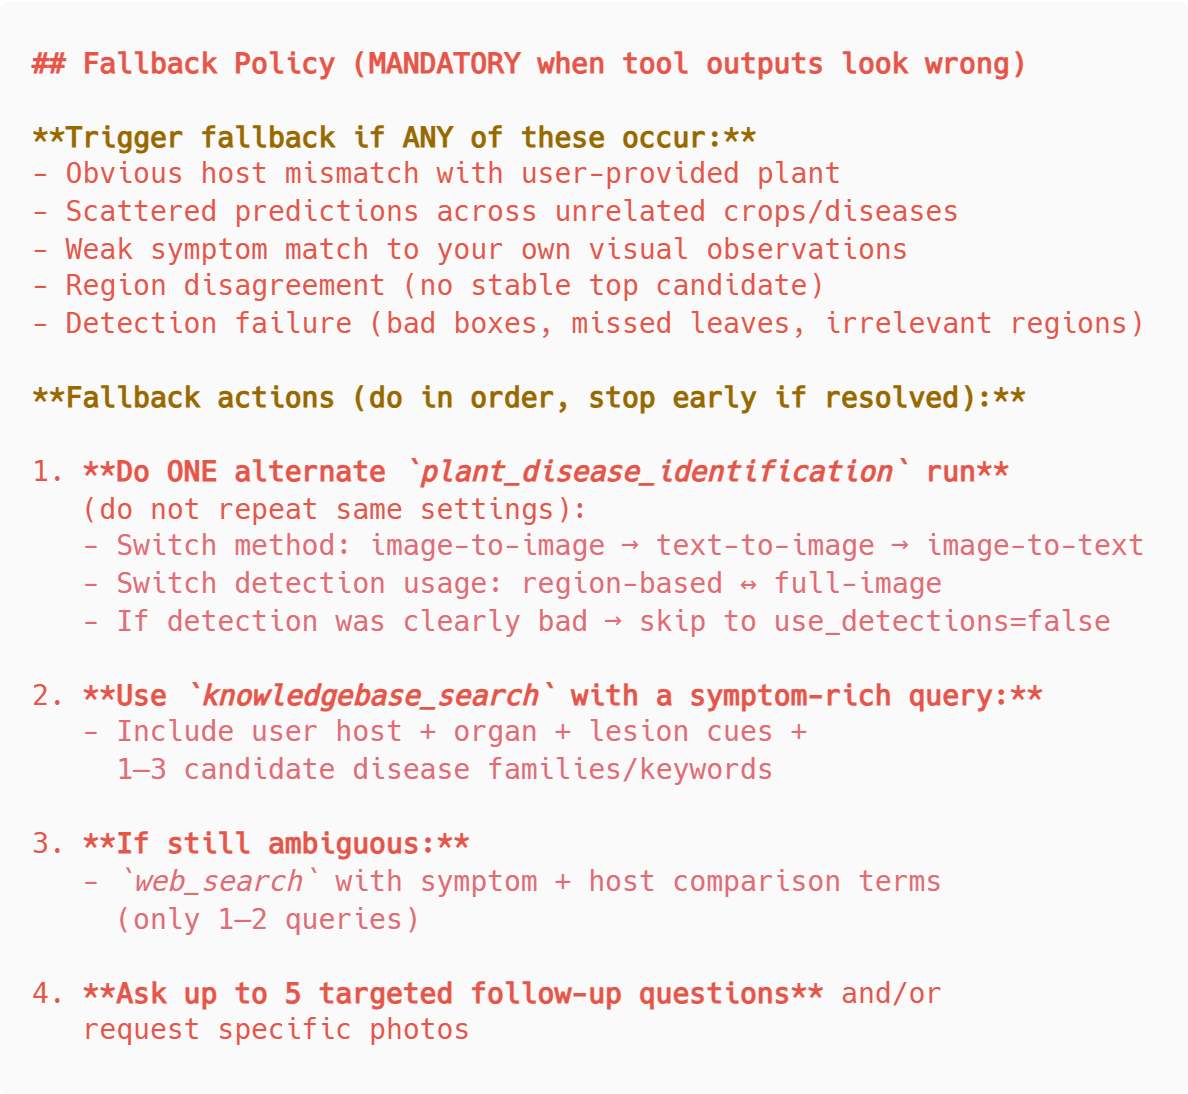
\includegraphics[width=\textwidth]{images/bab4/tool_decision_policy_4.png}
        \caption{}
    \end{subfigure}
    \caption[Realisasi \textit{tool decision policy} dalam instruksi sistem agen]{Realisasi \textit{tool decision policy} dalam instruksi sistem agen: (a) batasan global dan penyempitan berbasis basis pengetahuan, (b) dukungan visual dengan deteksi dan klasifikasi, (c) deteksi kosakata terbuka dan pemeriksaan keandalan pasca-klasifikasi, (d) kebijakan \textit{fallback}.}
    \label{fig:tool_decision_policy}
\end{figure}

Selain kebijakan penggunaan alat, agen juga mematuhi aturan kebenaran ketat (\textit{hard truthfulness rules}) yang berfungsi sebagai mekanisme anti-halusinasi. Aturan ini mewajibkan agen untuk selalu mendahulukan analisis visual (\textit{vision-first}) sebelum menggunakan alat, memisahkan antara observasi fakta dan inferensi dalam narasi, serta secara eksplisit menyebutkan sumber informasi (\textit{provenance}) untuk setiap klaim yang dibuat, misalnya "berdasarkan foto", "menurut hasil deteksi", atau "dari basis pengetahuan". Agen juga dilarang memberikan skor kepercayaan numerik buatan sendiri dan diwajibkan melakukan validasi silang antara hasil alat dengan konteks pengguna, misalnya berdasarkan inang dan gejala yang terlihat di citra. Jika pengguna meminta panduan penanganan, agen diwajibkan mencari bukti pendukung melalui pengambilan data sebelum memberikan saran spesifik. Realisasi bagian \textit{system prompt} ini diperlihatkan pada Gambar \ref{fig:hard_truthfulness}.

\begin{figure}[H]
    \centering
    \begin{subfigure}[t]{0.32\textwidth}
        \centering
        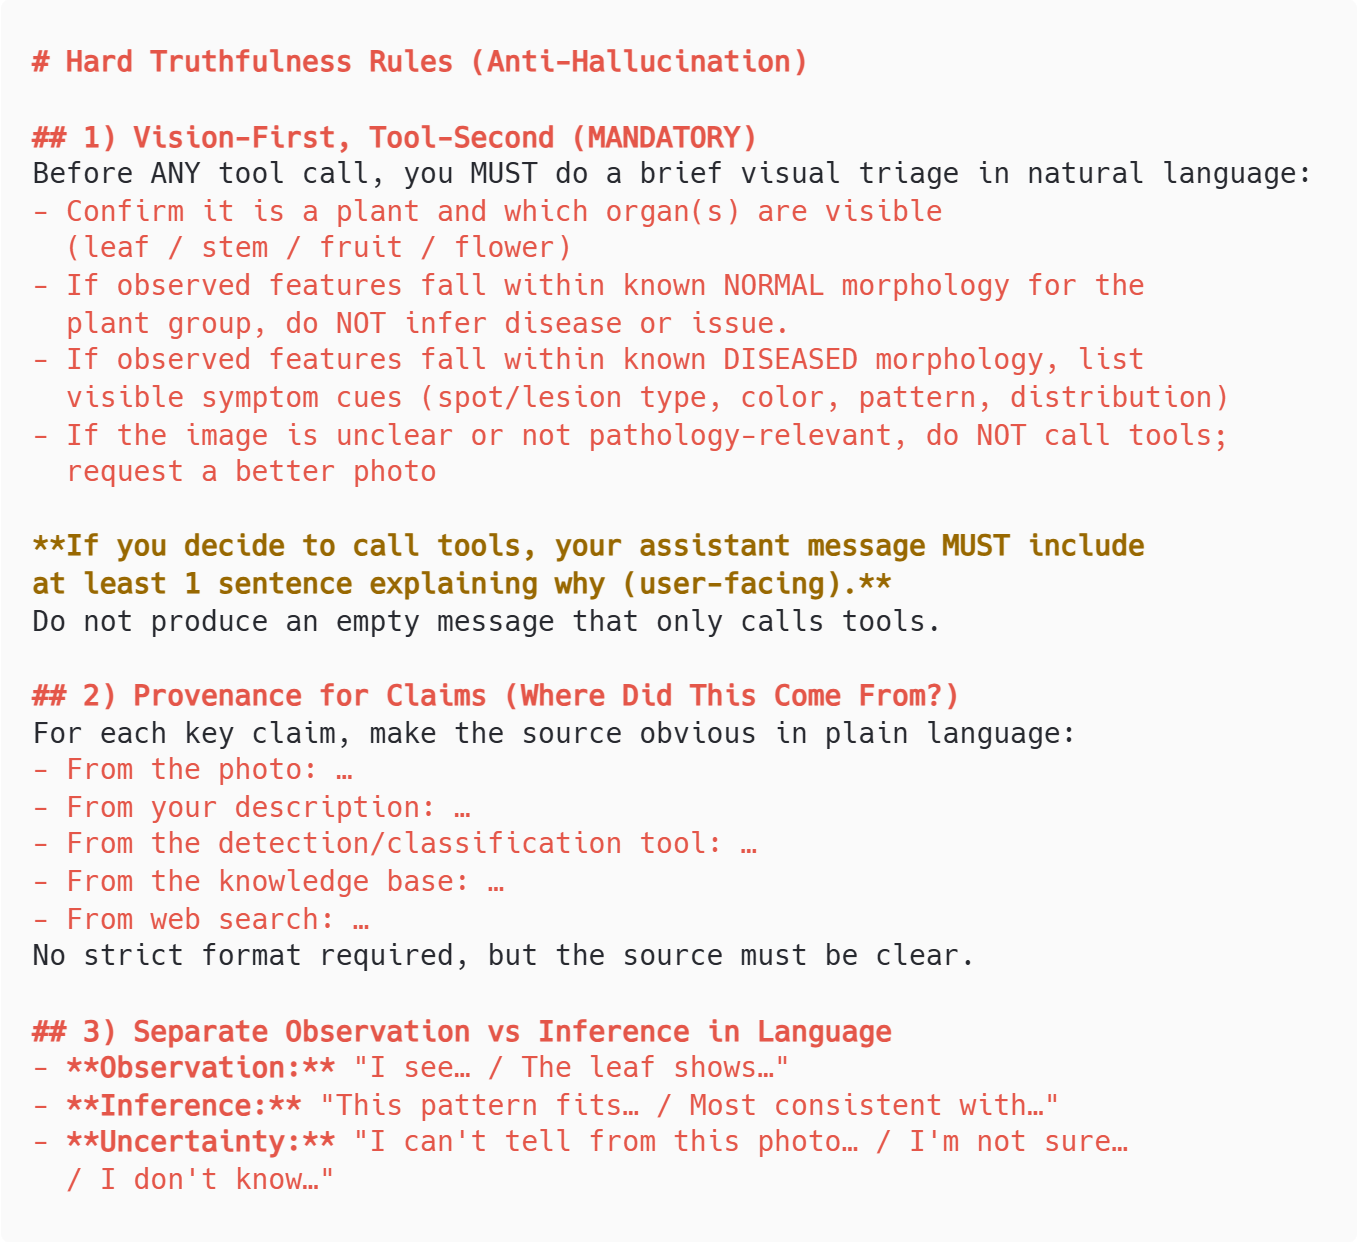
\includegraphics[width=\textwidth]{images/bab4/hard_truthfulness_1.png}
        \caption{}
    \end{subfigure}
    \hfill
    \begin{subfigure}[t]{0.32\textwidth}
        \centering
        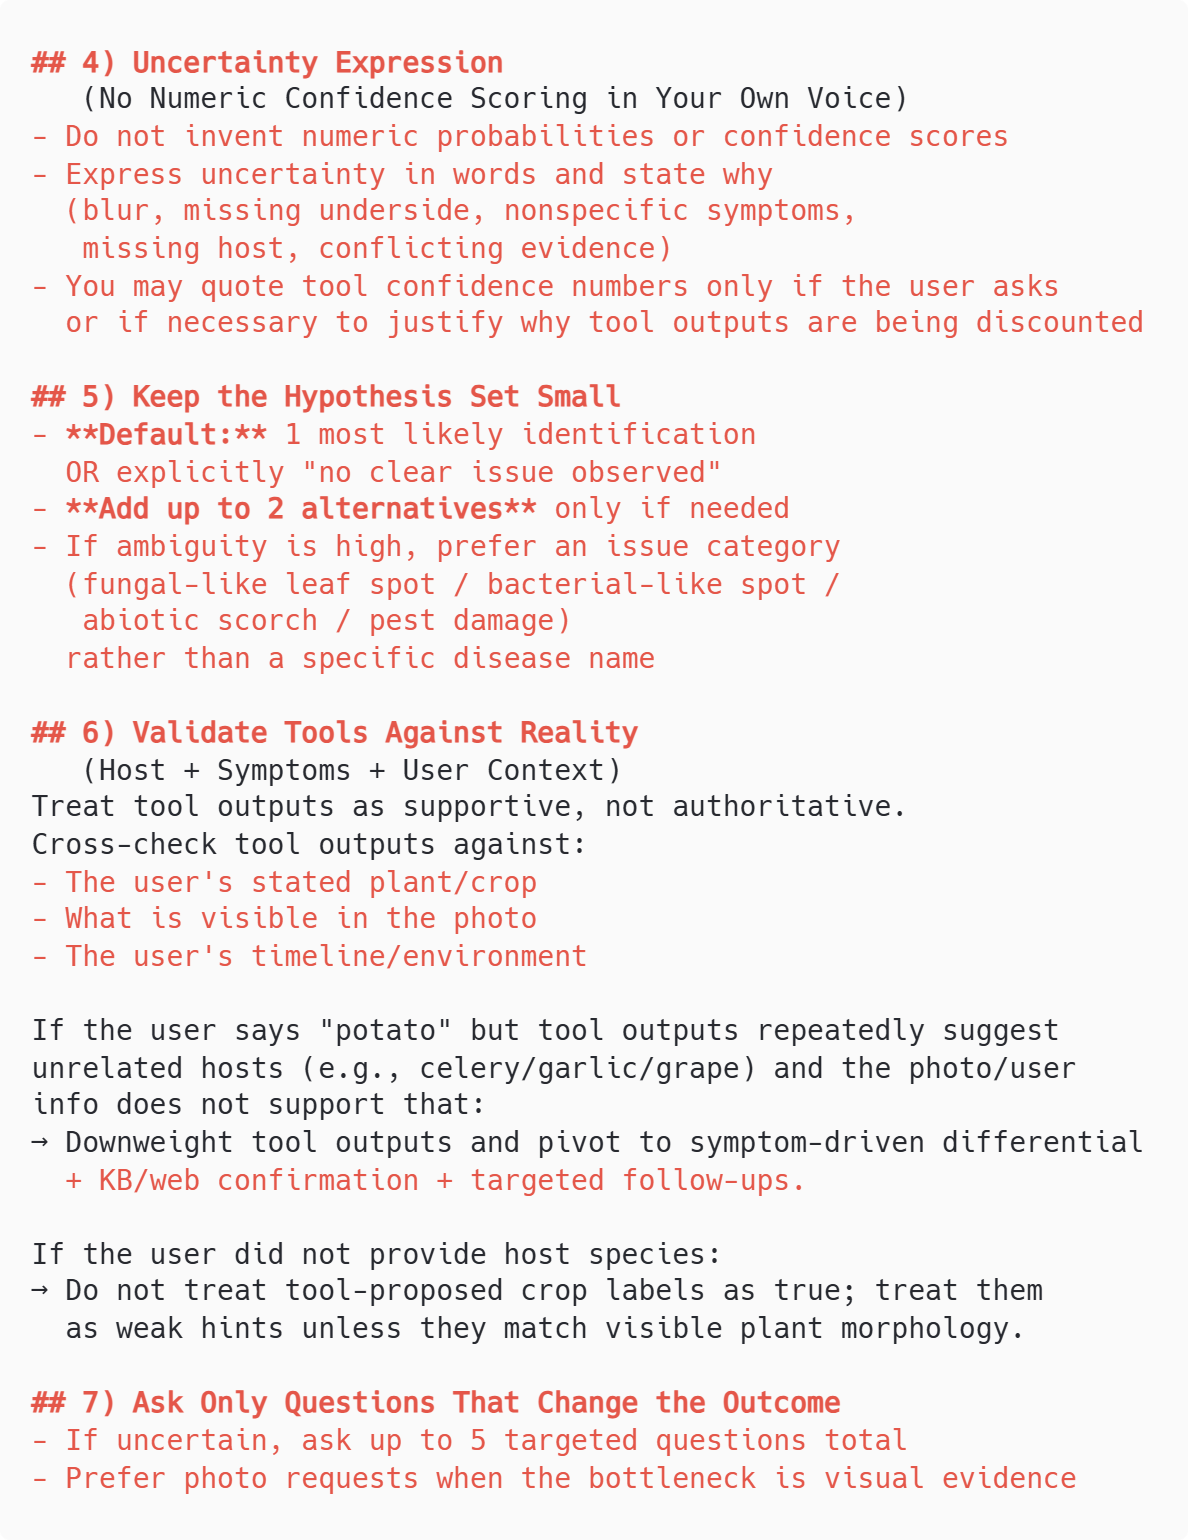
\includegraphics[width=\textwidth]{images/bab4/hard_truthfulness_2.png}
        \caption{}
    \end{subfigure}
    \hfill
    \begin{subfigure}[t]{0.32\textwidth}
        \centering
        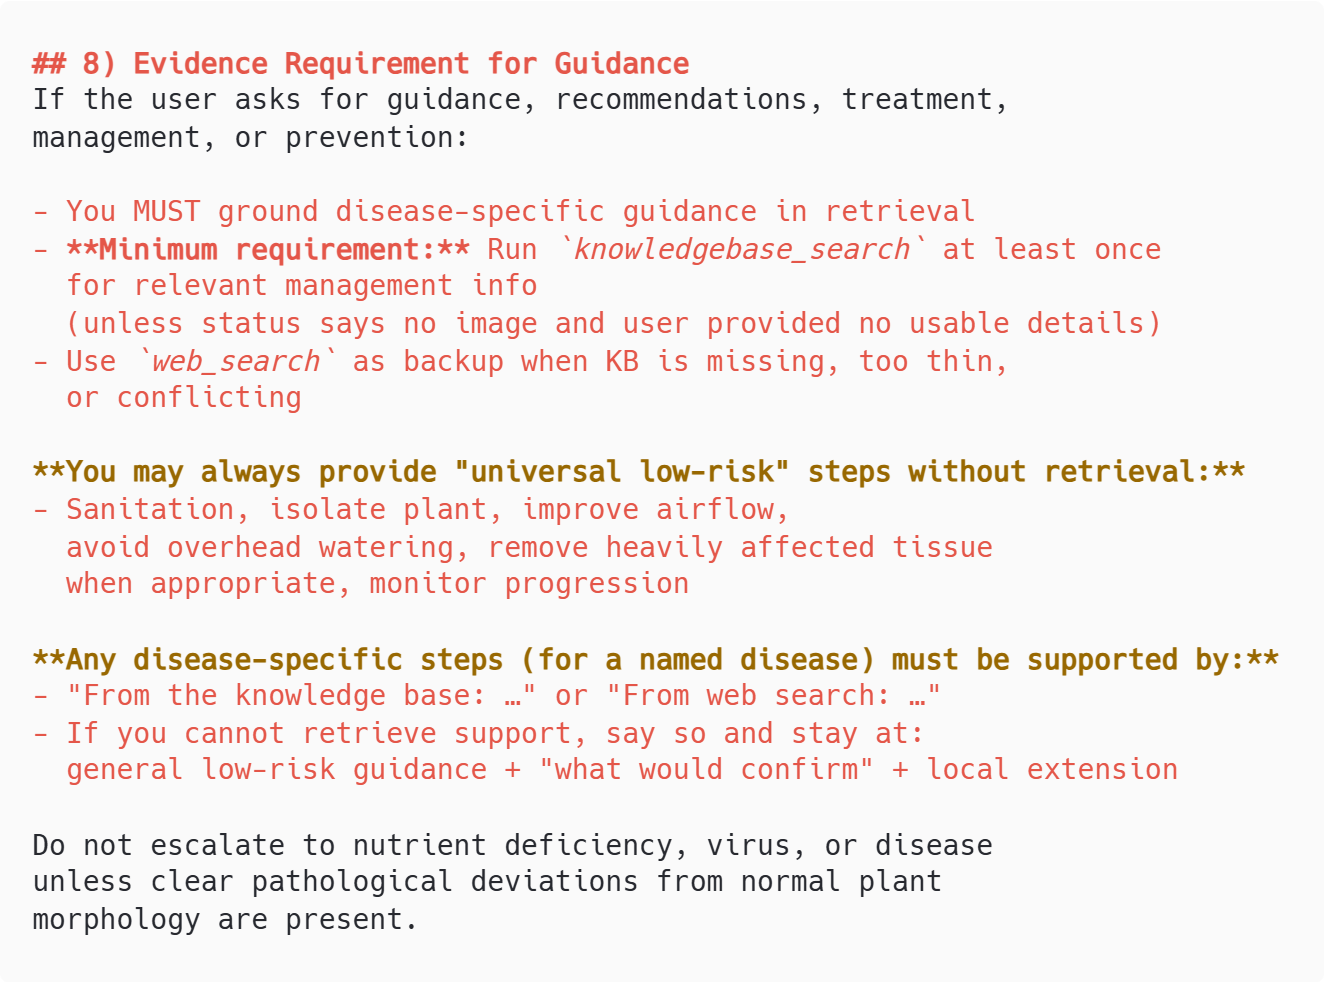
\includegraphics[width=\textwidth]{images/bab4/hard_truthfulness_3.png}
        \caption{}
    \end{subfigure}
    \caption[Realisasi \textit{hard truthfulness rules} pada instruksi sistem agen]{Realisasi \textit{hard truthfulness rules} pada instruksi sistem agen: (a) aturan analisis visual dan \textit{provenance} klaim, (b) ekspresi ketidakpastian dan validasi alat, (c) syarat pengambilan bukti untuk panduan penanganan}
    \label{fig:hard_truthfulness}
\end{figure}

\subsection{Modul Deteksi Objek}
Bagian ini memaparkan hasil evaluasi kinerja modul deteksi objek yang dirancang untuk mengidentifikasi keberadaan tanaman dalam citra. Pembahasan dibagi menjadi dua kategori berdasarkan dua alat deteksi yang digunakan, yaitu alat deteksi \textit{closed-set} daun menggunakan model YOLOv11 yang dilatih khusus, dan alat deteksi OVD untuk cakupan objek yang lebih luas menggunakan OWLv2 yang digunakan secara langsung.

\begin{enumerate}[label=\alph*., listparindent=\parindent, labelindent=0pt]
    \item Alat Deteksi \textit{Closed-Set} Daun

    Pelatihan model deteksi \textit{closed-set} dilaksanakan menggunakan lingkungan komputasi awan Kaggle Notebook yang didukung oleh akselerator GPU NVIDIA Tesla P100 dengan VRAM \qty{16}{\giga\byte}. Infrastruktur ini dipilih untuk menangani beban komputasi pelatihan model YOLOv11 yang intensif. Setelah pelatihan selesai, proses selanjutnya seperti evaluasi dan integrasi ke dalam sistem dilakukan pada perangkat keras lokal sesuai spesifikasi pada Tabel \ref{tab:perangkat_keras_pengembangan}. Sampel dataset PlantDoc yang dimodifikasi dengan menyatukan seluruh label kelas menjadi satu kelas tunggal "\textit{leaf}" untuk memfokuskan model pada tugas lokalisasi daun ditampilkan pada Gambar \ref{fig:dataset_plantdoc}.

    \noindent
    \begin{minipage}{\linewidth}
        \vspace{0.4cm}
        \captionsetup{type=figure}
        \centering
        
\includegraphics[width=0.8\textwidth]{bab4/datasetplantdoc.png}
        \caption[Sampel dataset PlantDoc]{Sampel citra dan anotasi dari dataset PlantDoc}
        \label{fig:dataset_plantdoc}
        \vspace{0.6cm}
    \end{minipage}

    Proses pelatihan dilakukan menggunakan kerangka kerja Ultralytics dengan konfigurasi hiperparameter yang disesuaikan. Tabel \ref{tab:training_hyperparams} merinci parameter-parameter kunci yang digunakan selama proses pelatihan untuk memastikan konvergensi model yang optimal. Nilai \textit{patience} sebesar 20 \textit{epoch} diterapkan agar proses pelatihan berhenti lebih awal apabila tidak terjadi peningkatan signifikan pada metrik validasi, sehingga waktu komputasi dapat digunakan lebih efisien. Pengaturan laju pembelajaran awal dan akhir yang sama (0.01) menandakan bahwa penjadwalan laju pembelajaran bersifat konstan selama pelatihan berlangsung.

    {
    \setstretch{1.0}
    \small
    \begin{longtblr}[
        caption = {Konfigurasi Hiperparameter Pelatihan Final},
        label = {tab:training_hyperparams},
    ]{
        width = \linewidth,
        colspec = {X[1.5,l] X[1,c]},
        hlines, vlines,
        rows = {m},
        row{1} = {font=\bfseries, halign=c, valign=m},
        rowhead = 1,
    }
        Parameter & Nilai \\
        Epochs & 240 \\
        Batch Size & 16 \\
        Image Size & $416 \times 416$ \\
        Optimizer & Auto \\
        Initial Learning Rate ($lr0$) & 0.01 \\
        Final Learning Rate ($lrf$) & 0.01 \\
        Momentum & 0.937 \\
        Weight Decay & 0.0005 \\
        Warmup Epochs & 3.0 \\
        Patience & 20 \\
    \end{longtblr}
    }

    Gambar \ref{fig:output_training_sample} memperlihatkan keluaran objek hasil pelatihan dari Ultralytics yang mencakup kurva evaluasi, metrik performa, dan statistik kecepatan inferensi. Objek tersebut memuat empat kurva evaluasi utama, yaitu \textit{Precision-Recall}, \textit{F1-Confidence}, \textit{Precision-Confidence}, dan \textit{Recall-Confidence}, yang dapat digunakan untuk menganalisis karakteristik detektor pada berbagai ambang kepercayaan. Keluaran ini juga menampilkan metrik ringkasan seperti mAP@50 dan mAP@50-95, serta statistik waktu yang mencakup tahap \textit{preprocess}, inferensi, dan \textit{postprocess}, sehingga memberikan gambaran menyeluruh mengenai kinerja model setelah pelatihan selesai.

    \noindent
    \begin{minipage}{\linewidth}
        \vspace{0.4cm}
        \captionsetup{type=figure}
        \centering
        
\includegraphics[width=0.8\textwidth]{bab4/outputhasiltraining.png}
        \caption[Sampel \textit{batch} pelatihan YOLOv11n]{Contoh sampel \textit{batch} pelatihan pada model YOLOv11n}
        \label{fig:output_training_sample}
        \vspace{0.6cm}
    \end{minipage}

    Untuk memfasilitasi integrasi sistem yang efisien dan mendukung interoperabilitas lintas platform, model deteksi daun yang telah dilatih dikonversi ke format ONNX (\textit{Open Neural Network Exchange}). Langkah ini diambil untuk memastikan model dapat dijalankan menggunakan \textit{runtime} teroptimasi (ONNX Runtime) pada lingkungan \textit{deployment} tanpa ketergantungan pada kerangka kerja pelatihan yang berat. Proses konversi dilakukan menggunakan fitur ekspor bawaan dari pustaka Ultralytics. Sebagaimana diperlihatkan pada Gambar \ref{fig:onnx_conversion_yolo}, proses ekspor berjalan sukses dengan validasi integritas model. Model ONNX yang dihasilkan memiliki spesifikasi input tensor citra berukuran $416 \times 416$ piksel dan menghasilkan output tensor yang memuat koordinat kotak pembatas serta skor probabilitas kelas untuk setiap deteksi.

    \noindent
    \begin{minipage}{\linewidth}
        \vspace{0.4cm}
        \captionsetup{type=figure}
        \centering
        \begin{subfigure}[b]{0.95\textwidth}
            \centering
            
\includegraphics[width=\textwidth]{bab4/proses_konversi_onnx_yolov11.png}
            \caption{}
            \label{fig:proses_onnx_yolo}
            \vspace{0.5cm}
        \end{subfigure}
        \begin{subfigure}[b]{0.95\textwidth}
            \centering
            
\includegraphics[width=\textwidth]{bab4/info_model_onnx_yolov11.png}
            \caption{}
            \label{fig:info_onnx_yolo}
        \end{subfigure}
        \caption[Konversi dan spesifikasi model ONNX YOLOv11]{Konversi dan spesifikasi model ONNX YOLOv11: (a) log proses ekspor model ke format ONNX, (b) ringkasan arsitektur input-output model}
        \label{fig:onnx_conversion_yolo}
        \vspace{0.6cm}
    \end{minipage}

    \item Alat \textit{Open-Vocabulary Object Detection}

    Komponen kedua dalam modul deteksi objek adalah alat \textit{Open-Vocabulary Object Detection} (OVD) yang bertugas menangani identifikasi objek dengan cakupan kategori yang lebih luas dan fleksibel. Untuk tujuan ini, digunakan model OWLv2 (\textit{Vision-Language Knowledge Distillation}) varian \textit{base-patch16-ensemble} dari Google yang tersedia secara publik. Agar kompatibel dengan arsitektur inferensi sistem yang seragam bersama detektor daun, model OWLv2 ini juga dikonversi ke format ONNX.

    Proses konversi dilakukan dengan memanfaatkan pustaka Optimum dari Hugging Face melalui optimum-cli. Konversi dijalankan dengan menetapkan tugas spesifik \textit{zero-shot-object-detection} untuk memastikan struktur graf komputasi yang sesuai. Gambar \ref{fig:onnx_conversion_owlv2} menampilkan proses ekspor yang berhasil memetakan model Transformer tersebut ke dalam format ONNX. Model hasil konversi menerima input \textit{multimodal} yang kompleks, terdiri dari \textit{pixel\_values} untuk representasi citra, serta \textit{input\_ids} dan \textit{attention\_mask} untuk representasi teks \textit{query}. Luaran model berupa tensor \textit{logits} dan \textit{pred\_boxes} yang merepresentasikan lokasi objek dan skor kesesuaian semantik terhadap \textit{query} teks yang diberikan.

    \noindent
    \begin{minipage}{\linewidth}
        \vspace{0.4cm}
        \captionsetup{type=figure}
        \centering
        \begin{subfigure}[b]{0.95\textwidth}
            \centering
            
\includegraphics[width=\textwidth]{bab4/proses_konversi_onnx_owlv2.png}
            \caption{}
            \label{fig:proses_onnx_owlv2}
            \vspace{0.2cm}
        \end{subfigure}
        \begin{subfigure}[b]{0.95\textwidth}
            \centering
            
\includegraphics[width=\textwidth]{bab4/info_model_onnx_owlv2.png}
            \caption{}
            \label{fig:info_onnx_owlv2}
        \end{subfigure}
        \caption[Konversi dan spesifikasi model ONNX OWLv2]{Konversi dan spesifikasi model ONNX OWLv2: (a) proses ekspor menggunakan Optimum CLI, (b) struktur input dan output model hasil konversi}
        \label{fig:onnx_conversion_owlv2}
        \vspace{0.6cm}
    \end{minipage}

\end{enumerate}

\subsection{Modul Pengambilan Informasi}
Bagian ini memaparkan hasil perancangan dan evaluasi dua komponen dalam modul pengambilan informasi, yaitu alat pengambilan citra-teks \textit{multimodal}, alat pengambilan basis pengetahuan yang menggabungkan \textit{hybrid search} dengan \textit{reranker}, dan alat pencarian internet yang memanfaatkan Tavily Search API.

\begin{enumerate}[label=\alph*., listparindent=\parindent, labelindent=0pt]
    \item Alat Pengambilan Citra-Teks

    Implementasi alat pengambilan citra-teks difokuskan pada pembangunan indeks vektor \textit{multimodal} yang mampu menangani \textit{query} lintas modal secara efisien. Proses ini mencakup tahapan \textit{ingestion} data ke dalam basis data vektor Qdrant serta verifikasi fungsionalitas teknik pengambilan yang telah dirancang. Proses \textit{ingestion} data PlantWild berhasil dilakukan dengan memetakan 18.275 pasang citra dan teks ke dalam koleksi Qdrant. Verifikasi pada dasbor Qdrant menunjukkan bahwa seluruh \textit{point} data telah terindeks dengan status "Green" (sehat), sebagaimana diperlihatkan pada Gambar \ref{fig:qdrant_collection}.

    \noindent
    \begin{minipage}{\linewidth}
        \vspace{0.4cm}
        \captionsetup{type=figure}
        \centering
        
\includegraphics[width=1\textwidth]{bab4/collectionplantwilddidashboardqdrant.png}
        \caption[Status koleksi data PlantWild pada Qdrant]{Tampilan dasbor Qdrant yang menunjukkan status koleksi data PlantWild}
        \label{fig:qdrant_collection}
        \vspace{0.6cm}
    \end{minipage}

    Setiap \textit{point} data menyimpan dua representasi vektor, yakni vektor citra dan teks yang dihasilkan oleh model SCOLD, serta \textit{payload} metadata yang mencakup nama tanaman, label penyakit, dan URL citra publik. Struktur data \textit{point} yang telah tersimpan divalidasi melalui inspeksi JSON pada antarmuka Qdrant seperti terlihat pada Gambar \ref{fig:qdrant_point}.

    \noindent
    \begin{minipage}{\linewidth}
        \vspace{0.4cm}
        \captionsetup{type=figure}
        \centering
        
\includegraphics[width=1\textwidth]{bab4/pointplantwildidashboardqdrant.png}
        \caption[Struktur \textit{point} data PlantWild]{Struktur \textit{point} data yang menyimpan vektor ganda dan metadata}
        \label{fig:qdrant_point}
        \vspace{0.6cm}
    \end{minipage}


    \item Alat Pengambilan Basis Pengetahuan

    Implementasi alat pengambilan basis pengetahuan difokuskan pada pembangunan indeks vektor yang mampu menangani strategi \textit{hybrid search} dengan dukungan berbagai model representasi. Proses \textit{ingestion} data melibatkan pemecahan dokumen menjadi segmen-segmen kecil yang kemudian dipetakan ke dalam ruang vektor menggunakan kombinasi model \textit{embedding} padat dan jarang. Hasil dari proses ini adalah terbentuknya koleksi "knowledgebase\_collection" pada basis data vektor Qdrant yang berisi 2.458 \textit{point} data pengetahuan penyakit tanaman. Status indeks yang sehat diverifikasi melalui dasbor Qdrant yang menampilkan indikator "Green" pada koleksi tersebut, sebagaimana diperlihatkan pada Gambar \ref{fig:qdrant_kb_collection}.

    \noindent
    \begin{minipage}{\linewidth}
        \vspace{0.4cm}
        \captionsetup{type=figure}
        \centering
        
\includegraphics[width=0.8\textwidth]{bab4/knowledgebase_collection_index.png}
        \caption[Status koleksi basis pengetahuan pada Qdrant]{Tampilan dasbor Qdrant untuk koleksi basis pengetahuan dengan konfigurasi multi-vektor}
        \label{fig:qdrant_kb_collection}
        \vspace{0.6cm}
    \end{minipage}

    Setiap \textit{point} dalam koleksi tersebut menyimpan representasi vektor yang majemuk untuk mengakomodasi kebutuhan pencarian semantik dan leksikal secara bersamaan. Vektor-vektor yang disimpan meliputi keluaran dari model text-embedding-3-large, gemini-embedding-001, jina-colbert-v2, splade, dan bm25. Di samping data vektor, struktur \textit{point} juga memuat \textit{payload} metadata yang kaya informasi, seperti kategori penyakit, nama tanaman inang, dan sumber referensi asli. Validasi terhadap kelengkapan struktur data ini dilakukan melalui fitur inspeksi \textit{point} pada antarmuka Qdrant seperti yang tampak pada Gambar \ref{fig:qdrant_kb_point}.

    \noindent
    \begin{minipage}{\linewidth}
        \vspace{0.4cm}
        \captionsetup{type=figure}
        \centering
        
\includegraphics[width=0.8\textwidth]{bab4/knowledgebase_point.png}
        \caption[Struktur \textit{point} basis pengetahuan]{Detail struktur \textit{point} pada basis pengetahuan yang memuat vektor hibrida dan metadata}
        \label{fig:qdrant_kb_point}
        \vspace{0.6cm}
    \end{minipage}


    \item Alat Pencarian Internet

    Pengintegrasian alat pencarian internet ke dalam sistem agentik menggunakan Tavily Search API sebagai penyedia layanan pencarian berbasis web yang dirancang untuk kebutuhan agen LLM. Proses konfigurasi dimulai dengan pembuatan akun pada halaman web layanan Tavily, yang kemudian dilanjutkan dengan pembuatan API key melalui dasbor akun, seperti yang terlihat pada Gambar~\ref{fig:tavily_dashboard}. API key tersebut selanjutnya diberikan sebagai argumen saat membuat instance integrasi Tavily dengan LangChain, sehingga agen dapat memanggil alat pencarian ini secara langsung dalam alur kerjanya.

    \noindent
    \begin{minipage}{\linewidth}
        \vspace{0.4cm}
        \captionsetup{type=figure}
        \centering
        
\includegraphics[width=0.85\textwidth]{bab4/tampilan_halaman_web_tavily.png}
        \caption[Dasbor layanan Tavily]{Tampilan dasbor layanan Tavily berisi API key yang digunakan untuk integrasi}
        \label{fig:tavily_dashboard}
        \vspace{0.6cm}
    \end{minipage}

\end{enumerate}


\subsection{Antarmuka Sistem Agentik}
Implementasi antarmuka sistem berbasis web telah berhasil mengintegrasikan seluruh kapabilitas agen ke dalam pengalaman pengguna yang intuitif. Antarmuka ini dirancang untuk memfasilitasi interaksi natural antara pengguna dan agen cerdas, mendukung input \textit{multimodal} berupa teks dan citra, serta menyediakan transparansi langkah agen (\textit{thought process}) yang dapat diakses pengguna. Tampilan utama antarmuka sistem yang telah dikembangkan disajikan pada Gambar \ref{fig:hasil_antarmuka}.

\begin{figure}[H]
    \centering
    
\includegraphics[width=1\textwidth]{bab4/hasilantarmuka.png}
    \caption[Antarmuka utama sistem agentik]{Tampilan antarmuka utama sistem agentik}
    \label{fig:hasil_antarmuka}
\end{figure}

Sistem juga telah didistribusikan ke lingkungan produksi untuk memvalidasi aksesibilitasnya secara publik. Komponen antarmuka pengguna (\textit{frontend}) telah berhasil dikerahkan ke layanan \textit{hosting} Vercel, sehingga dapat diakses oleh pengguna melalui peramban web di internet. Di sisi \textit{backend}, sistem agentik telah dikontainerisasi dalam \textit{image} Docker dan dijalankan pada infrastruktur \textit{serverless} Google Cloud Run. Gambar \ref{fig:interface_vercel} menampilkan status \textit{deployment} antarmuka pada dasbor Vercel, sedangkan Gambar \ref{fig:agent_cloud_run} memperlihatkan layanan kontainer sistem agentik yang telah aktif di Google Cloud Run.

\begin{figure}[H]
    \centering
    \begin{subfigure}[b]{0.8\textwidth}
        \centering
        
\includegraphics[width=\textwidth]{bab4/interface_vercel.png}
        \caption[Status \textit{deployment} antarmuka]{Status \textit{deployment} antarmuka pengguna pada platform Vercel}
        \label{fig:interface_vercel}
        \vspace{0.4cm}
    \end{subfigure}
    \begin{subfigure}[b]{0.8\textwidth}
        \centering
        
\includegraphics[width=\textwidth]{bab4/agent_cloud_run.png}
        \caption[Layanan kontainer sistem agentik]{Layanan kontainer sistem agentik yang berjalan pada Google Cloud Run}
        \label{fig:agent_cloud_run}
    \end{subfigure}
    \caption[Status \textit{deployment} sistem]{Status \textit{deployment} sistem pada lingkungan produksi}
    \label{fig:production_deployment}
\end{figure}


\section{Hasil Pengujian dan Evaluasi}

Evaluasi kinerja sistem dilakukan melalui serangkaian pengujian yang terstruktur untuk memvalidasi keandalan dan efektivitas solusi yang diusulkan. Proses pengujian ini mencakup verifikasi fungsionalitas dan pengukuran kinerja pada setiap komponen utama penyusun sistem. Pemaparan hasil evaluasi diawali dengan analisis kinerja modul deteksi objek yang meliputi akurasi dan efisiensi komputasi model deteksi. Selanjutnya, evaluasi dilakukan pada modul pengambilan informasi untuk menilai efektivitas strategi pencarian yang diterapkan. Pengujian juga mencakup aspek antarmuka pengguna guna memastikan kegunaan sistem. Puncak dari rangkaian evaluasi ini adalah pengujian sistem agentik secara menyeluruh (\textit{end-to-end}) yang mengukur kemampuan agen dalam menyelesaikan tugas diagnostik dan interaksi percakapan dalam berbagai skenario uji.

\subsection{Modul Deteksi Objek}

Pengujian dan evaluasi kinerja modul deteksi objek dilakukan untuk memvalidasi kemampuan sistem dalam mengidentifikasi objek tanaman secara akurat dan efisien. Pengujian ini mencakup analisis mendalam terhadap dua komponen utama, yaitu alat deteksi \textit{closed-set} yang berfokus pada daun menggunakan model YOLOv11 dan alat deteksi \textit{open-vocabulary} menggunakan model OWLv2 untuk cakupan objek yang lebih luas. Selain itu, pengujian juga mencakup pengujian integrasi kedua alat deteksi tersebut dalam konteks sistem agentik untuk memastikan operabilitas yang optimal dalam skenario penggunaan nyata.

\begin{enumerate}[label=\alph*., listparindent=\parindent, labelindent=0pt]
    \item Alat Deteksi \textit{Closed-Set} Daun

    Kinerja pelatihan ketiga varian model, yaitu YOLOv11n, YOLOv11s, dan YOLOv11m, dipantau melalui kurva \textit{loss} dan metrik validasi. Sebagaimana diperlihatkan pada Gambar \ref{fig:training_curves}, ketiga model menunjukkan tren penurunan \textit{loss} yang stabil dan peningkatan metrik mAP yang konsisten seiring bertambahnya \textit{epoch}. Tidak terlihat indikasi \textit{overfitting} yang signifikan pada ketiga varian, yang mengindikasikan bahwa konfigurasi pemodelan diterapkan selama pelatihan bekerja dengan baik.

    \noindent
    \begin{minipage}{\linewidth}
        \vspace{0.4cm}
        \captionsetup{type=figure}
        \centering
        \begin{subfigure}[b]{0.45\textwidth}
            \centering
            
\includegraphics[width=\textwidth]{bab4/yolov11ntraningcurve.png}
            \caption{}
        \end{subfigure}
        \hfill
        \begin{subfigure}[b]{0.45\textwidth}
            \centering
            
\includegraphics[width=\textwidth]{bab4/yolov11straningcurve.png}
            \caption{}
        \end{subfigure}
        
        \vspace{0.2cm}

        \begin{subfigure}[b]{0.45\textwidth}
            \centering
            
\includegraphics[width=\textwidth]{bab4/yolov11mtraningcurve.png}
            \caption{}
        \end{subfigure}
        \caption[Kurva pelatihan dan validasi varian YOLOv11]{Kurva metrik pelatihan dan validasi untuk model (a) YOLOv11n, (b) YOLOv11s, dan (c) YOLOv11m}
        \label{fig:training_curves}
        \vspace{0.6cm}
    \end{minipage}

    Kemampuan generalisasi model pada data yang belum pernah dilihat sebelumnya diuji secara kualitatif. Gambar \ref{fig:test_predictions} menampilkan hasil prediksi deteksi daun pada data uji untuk ketiga varian model. Hasil visual menunjukkan bahwa ketiga model mampu mendeteksi dan melokalisasi daun dengan tingkat kepercayaan yang tinggi pada berbagai kondisi citra. Analisis lebih lanjut terhadap hasil prediksi memperlihatkan bahwa model mampu menangani tantangan oklusi dan variasi skala dengan baik. Daun yang saling bertumpuk atau yang memiliki tekstur permukaan tidak seragam akibat gejala penyakit tetap dapat diidentifikasi sebagai objek tunggal yang utuh. Selain itu, tingginya skor kepercayaan (\textit{confidence score}) pada sebagian besar deteksi mengindikasikan bahwa fitur-fitur yang dipelajari model cukup diskriminatif untuk membedakan objek daun dari latar belakang yang kompleks.

    \noindent
    \begin{minipage}{\linewidth}
        \vspace{0.6cm}
        \captionsetup{type=figure}
        \centering
        \begin{subfigure}[b]{0.45\textwidth}
            \centering
            
\includegraphics[width=\textwidth]{bab4/testprediksiyolov11n.png}
            \caption{}
        \end{subfigure}
        \hfill
        \begin{subfigure}[b]{0.45\textwidth}
            \centering
            
\includegraphics[width=\textwidth]{bab4/testprediksiyolov11s.png}
            \caption{}
        \end{subfigure}
        
        \vspace{0.5cm}

        \begin{subfigure}[b]{0.45\textwidth}
            \centering
            
\includegraphics[width=\textwidth]{bab4/testprediksiyolov11m.png}
            \caption{}
        \end{subfigure}
        \caption[Hasil prediksi deteksi daun pada data uji]{Hasil prediksi deteksi daun pada data uji menggunakan model (a) YOLOv11n, (b) YOLOv11s, dan (c) YOLOv11m}
        \label{fig:test_predictions}
        \vspace{0.6cm}
    \end{minipage}

    Evaluasi kuantitatif lebih lanjut dilakukan melalui pengujian ketiga varian model pada dataset uji PlantDoc untuk memperoleh metrik akurasi deteksi dan efisiensi komputasi. Pengujian ini mencakup dua aspek utama, yaitu akurasi yang diukur menggunakan mAP@50 dan mAP@50-95, serta efisiensi yang diukur melalui latensi inferensi pada lingkungan CPU. Rangkuman hasil \textit{benchmarking} performa ketiga model tersebut disajikan dalam Tabel \ref{tab:yolo_results}.

    {
    \setstretch{1.0}
    \small
    \begin{longtblr}[
        caption = {Rangkuman Hasil Evaluasi Performa dan Latensi Model YOLOv11},
        entry = {Hasil Evaluasi Performa dan Latensi YOLOv11},
        label = {tab:yolo_results},
    ]{
        width = \linewidth,
        colspec = {*{5}{X[c]}},
        hlines, vlines,
        rows = {m},
        row{1} = {font=\bfseries, halign=c, valign=m},
        rowhead = 1,
        rowsep = 3pt,
    }
        Varian & mAP@50 & mAP@50-95 & Latensi p50 (ms) & Latensi p95 (ms) \\
        YOLOv11n & 0.8800 & 0.6953 & 10.47 & 12.69 \\
        YOLOv11s & 0.8916 & 0.7105 & 21.35 & 27.33 \\
        YOLOv11m & 0.8976 & 0.7071 & 55.83 & 67.19 \\
    \end{longtblr}
    }

    Berdasarkan metrik akurasi deteksi, seluruh varian model menunjukkan performa yang kompetitif dengan skor mAP@50 di atas 0.88. Sebagaimana diilustrasikan pada Gambar \ref{fig:yolo_performance}, YOLOv11m mencatatkan skor mAP@50 tertinggi sebesar 0.8976, namun pada metrik mAP@50-95 yang lebih ketat, YOLOv11s justru mengungguli YOLOv11m dengan skor 0.7105 berbanding 0.7071. Hal ini mengindikasikan bahwa peningkatan kompleksitas model pada YOLOv11m tidak serta-merta menjamin peningkatan akurasi lokalisasi yang signifikan dibandingkan YOLOv11s. YOLOv11n, walaupun memiliki arsitektur terkecil, tetap mampu memberikan performa yang solid dengan selisih akurasi yang relatif kecil dibandingkan varian yang lebih besar.

    \noindent
    \begin{minipage}{\linewidth}
        \vspace{0.4cm}
        \captionsetup{type=figure}
        \centering
        
\includegraphics[width=0.8\textwidth]{bab4/perbandingan_performa_yolov11.png}
        \caption[Perbandingan performa varian YOLOv11]{Perbandingan performa deteksi (mAP) antar varian YOLOv11}
        \label{fig:yolo_performance}
        \vspace{0.6cm}
    \end{minipage}

    Setelah proses pelatihan selesai, model yang telah diekspor ke format ONNX dilakukan proses \textit{benchmarking} latensi guna mengevaluasi kecepatan inferensi model pada perangkat keras lokal sesuai spesifikasi yang tercantum dalam Tabel \ref{tab:perangkat_pengembangan}. Proses berjalan pada sistem operasi Windows 11 Home Single Language 25H2 dengan \textit{Build} 26200.7840. Pengujian ini memanfaatkan \textit{engine} \textit{onnxruntime} versi 1.24.3 dengan konfigurasi eksekusi menggunakan 8 \textit{core} fisik yang tersedia dan dibatasi pada 1 \textit{thread} agar CPU fokus pada satu tugas. Proses pengukuran dilakukan sebanyak 3 kali pengulangan untuk setiap skenario pengujian, kemudian hasil akhirnya diambil dari nilai rata-ratanya guna meminimalkan bias akibat fluktuasi sesaat pada sistem. Seluruh rangkaian \textit{benchmarking} dilaksanakan dalam kondisi lingkungan yang terkontrol, di mana proses latar belakang sistem diminimalkan untuk mensanitasi lingkungan pengujian dari variabilitas beban kerja eksternal. Dokumentasi proses eksekusi \textit{benchmarking} tersebut ditampilkan pada Gambar \ref{fig:proses_benchmark_latensi}.

    \noindent
    \begin{minipage}{\linewidth}
        \vspace{0.4cm}
        \captionsetup{type=figure}
        \centering
        
\includegraphics[width=1\textwidth]{bab4/proses_benchmark_latensi.png}
        \caption[Proses \textit{benchmarking} latensi model ONNX]{Tampilan proses \textit{benchmarking} latensi model ONNX}
        \label{fig:proses_benchmark_latensi}
        \vspace{0.6cm}
    \end{minipage}

    Dari sisi efisiensi komputasi, terdapat perbedaan latensi yang signifikan antar ketiga varian model saat dijalankan pada lingkungan CPU. Gambar \ref{fig:yolo_latency} memperlihatkan bahwa YOLOv11n merupakan model tercepat dengan latensi median (p50) hanya 10.47 ms, menjadikannya sangat responsif untuk aplikasi \textit{real-time}. YOLOv11s memiliki latensi sekitar dua kali lipat lebih tinggi sebesar 21.35 ms, sedangkan YOLOv11m mengalami lonjakan latensi yang drastis hingga 55.83 ms. Latensi p95 juga menunjukkan tren serupa, menegaskan stabilitas waktu inferensi masing-masing model.

    \noindent
    \begin{minipage}{\linewidth}
        \vspace{0.4cm}
        \captionsetup{type=figure}
        \centering
        
\includegraphics[width=0.8\textwidth]{bab4/perbandingan_latensi_yolov11.png}
        \caption[Perbandingan latensi varian YOLOv11]{Perbandingan latensi inferensi (p50 dan p95) antar varian YOLOv11}
        \label{fig:yolo_latency}
        \vspace{0.6cm}
    \end{minipage}

    Untuk menentukan model yang paling optimal, dilakukan analisis \textit{Pareto frontier} yang memetakan hubungan \textit{trade-off} antara akurasi dan kecepatan. Gambar \ref{fig:pareto_analysis} menampilkan kurva Pareto untuk dua skenario metrik. Pada grafik mAP@50 berbanding Latensi p50 pada Gambar \ref{fig:pareto_map50}, terlihat adanya keuntungan marjinal yang semakin mengecil saat beralih dari varian YOLOv11s ke YOLOv11m. Sementara itu, pada grafik mAP@50-95 berbanding Latensi p95 pada Gambar \ref{fig:pareto_map5095}, varian YOLOv11m terlihat berada di bawah garis efisiensi karena memiliki akurasi yang lebih rendah dibanding YOLOv11s namun dengan latensi yang jauh lebih tinggi. Berdasarkan analisis ini, YOLOv11n dinilai sebagai pilihan terbaik untuk skenario yang memprioritaskan kecepatan ekstrem, sedangkan YOLOv11s menawarkan keseimbangan terbaik antara akurasi tinggi dan latensi yang masih dapat diterima. Oleh karena itu, varian YOLOv11s dipilih sebagai model yang akan diintegrasikan ke dalam alat deteksi \textit{closed-set} pada sistem agentik yang dikembangkan.

    \noindent
    \begin{minipage}{\linewidth}
        \vspace{0.4cm}
        \captionsetup{type=figure}
        \centering
        \begin{subfigure}[b]{0.8\textwidth}
            \centering
            
\includegraphics[width=\textwidth]{bab4/pareto_frontier_map50_latensip50.png}
            \caption{}
            \label{fig:pareto_map50}
        \end{subfigure}
        \par\bigskip
        \begin{subfigure}[b]{0.8\textwidth}
            \centering
            
\includegraphics[width=\textwidth]{bab4/pareto_frontier_map5095_latensi_p95.png}
            \caption{}
            \label{fig:pareto_map5095}
        \end{subfigure}
        \caption[Analisis \textit{Pareto Frontier} untuk pemilihan model]{Analisis \textit{Pareto Frontier} pada (a) mAP@50 vs Latensi p50 dan (b) mAP@50-95 vs Latensi p95 untuk pemilihan model terbaik}
        \label{fig:pareto_analysis}
        \vspace{0.6cm}
    \end{minipage}

    \item Alat \textit{Open-Vocabulary Object Detection}

    Evaluasi pengujian kualitatif terhadap alat OVD (\textit{Open-Vocabulary Object Detection}) menggunakan model OWLv2 menunjukkan kemampuan model dalam mendeteksi objek tanaman selain daun, seperti buah, berdasarkan instruksi teks (\textit{text prompt}). Gambar \ref{fig:owlv2_detection} menampilkan contoh hasil deteksi di mana model berhasil mengidentifikasi dan melokalisasi buah apel ketika diberikan \textit{prompt} "fruit". Kemampuan ini memberikan fleksibilitas bagi sistem untuk menganalisis berbagai organ tanaman tanpa perlu melatih ulang model untuk setiap kelas objek baru.

    \noindent
    \begin{minipage}{\linewidth}
        \vspace{0.4cm}
        \captionsetup{type=figure}
        \centering
        
\includegraphics[width=0.8\textwidth]{bab4/deteksiowlv2.png}
        \caption[Hasil deteksi buah dengan OWLv2]{Contoh hasil deteksi buah menggunakan model OWLv2}
        \label{fig:owlv2_detection}
        \vspace{0.6cm}
    \end{minipage}

    Untuk memvalidasi secara empiris bahwa model OWLv2 memiliki beban komputasi yang berat, dilakukan pengujian latensi sederhana sebagai pembanding terhadap YOLOv11. Mengingat waktu inferensi model yang lambat, pengujian latensi untuk OWLv2 ini hanya dilakukan dengan satu kali proses pengukuran yang terdiri dari 10 iterasi pemanasan dan 100 iterasi utama. Keterbatasan jumlah iterasi ini diterapkan untuk mengefisiensikan waktu pengujian karena satu siklus inferensi memakan waktu yang cukup signifikan. Dokumentasi proses pengukuran latensi untuk model OWLv2 ini ditampilkan pada Gambar \ref{fig:proses_latensi_owlv2}.

    \noindent
    \begin{minipage}{\linewidth}
        \vspace{0.4cm}
        \captionsetup{type=figure}
        \centering
        
\includegraphics[width=1\textwidth]{bab4/proses_lantensi_owlv2.png}
        \caption[Proses pengukuran latensi OWLv2]{Tampilan proses pengukuran latensi OWLv2}
        \label{fig:proses_latensi_owlv2}
        \vspace{0.6cm}
    \end{minipage}

    Perbandingan latensi antara alat deteksi \textit{closed-set} daun dengan YOLOv11 dan OVD dengan OWLv2 disajikan secara lengkap pada Tabel \ref{tab:latency_comparison}. Data menunjukkan disparitas performa yang sangat signifikan, di mana OWLv2 lebih lambat hingga ratusan kali lipat dibandingkan varian model YOLOv11. Meskipun demikian, latensi sekitar 2,3 detik ini dinilai masih berada dalam batas toleransi yang dapat diterima untuk sebuah sistem agen interaktif, terutama mengingat peran OWLv2 yang diposisikan sebagai alat spesialis untuk skenario yang lebih fleksibel, bukan sebagai alat deteksi utama yang dipanggil pada setiap interaksi.

    {
    \setstretch{1.0}
    \small
    \begin{longtblr}[
        caption = {Perbandingan Latensi Model Deteksi YOLOv11 dan OWLv2},
        label = {tab:latency_comparison},
    ]{
        width = \linewidth,
        colspec = {X[1,c] X[1,c] X[1,c]},
        hlines, vlines,
        rows = {m},
        row{1} = {font=\bfseries, halign=c, valign=m},
        rowhead = 1,
    }
        Model & Latensi p50 (ms) & Latensi p95 (ms) \\
        YOLOv11n & 10,47 & 12,69 \\
        YOLOv11s & 21,35 & 27,33 \\
        YOLOv11m & 55,83 & 67,19 \\
        OWLv2 & 2275,33 & 2352,31 \\
    \end{longtblr}
    }

    \end{enumerate}

    Setelah memverifikasi kinerja model dari masing-masing alat, tahap selanjutnya adalah memastikan bahwa kedua alat deteksi tersebut dapat beroperasi secara optimal dalam ekosistem sistem yang terintegrasi. Pengujian integrasi fungsional ini bertujuan untuk memvalidasi operabilitas alat, baik saat dijalankan secara mandiri sebagai fungsi terisolasi maupun ketika dipanggil secara dinamis oleh agen berdasarkan instruksi pengguna. Pengujian awal dilakukan secara terisolasi dengan menjalankan kode pemanggilan fungsi alat deteksi \textit{closed-set} daun dan alat OVD secara langsung tanpa melibatkan agen. Sebagaimana diperlihatkan pada Gambar \ref{fig:isolated_tests}, kedua alat berhasil dijalankan dan menghasilkan luaran deteksi yang sesuai dengan harapan, baik untuk deteksi daun maupun deteksi objek terbuka seperti buah.

    \begin{figure}[H]
        \centering
        \begin{subfigure}[b]{0.45\textwidth}
            \centering
            
\includegraphics[width=\textwidth]{bab4/kode_pengujian_csod.png}
            \caption{}
            \label{fig:code_csod}
        \end{subfigure}
        \hfill
        \begin{subfigure}[b]{0.45\textwidth}
            \centering
            
\includegraphics[width=\textwidth]{bab4/keluaran_pengujian_csod.png}
            \caption{}
            \label{fig:output_csod}
        \end{subfigure}
        
        \vspace{0.4cm}

        \begin{subfigure}[b]{0.45\textwidth}
            \centering
            
\includegraphics[width=\textwidth]{bab4/kode_pengujian_ovd.png}
            \caption{}
            \label{fig:code_ovd}
        \end{subfigure}
        \hfill
        \begin{subfigure}[b]{0.45\textwidth}
            \centering
            
\includegraphics[width=\textwidth]{bab4/keluaran_pengujian_ovd.png}
            \caption{}
            \label{fig:output_ovd}
        \end{subfigure}
        \caption[Pengujian terisolasi alat deteksi]{Pengujian terisolasi alat deteksi: (a) kode pengujian deteksi \textit{closed-set} daun, (b) luaran deteksi \textit{closed-set} daun, (c) kode pengujian OVD, dan (d) luaran deteksi OVD}
        \label{fig:isolated_tests}
    \end{figure}

    Selanjutnya, pengujian dilakukan dengan mengintegrasikan alat-alat tersebut ke dalam sistem agen untuk memvalidasi kemampuan agen dalam memilih dan menggunakan alat yang tepat berdasarkan instruksi bahasa alami. Pada tahap ini, agen diberikan instruksi spesifik untuk mendeteksi daun dan buah pada citra yang diberikan. Gambar \ref{fig:integration_tests} menampilkan jejak eksekusi pada LangSmith yang menunjukkan bahwa agen mampu menafsirkan instruksi pada \textit{prompt}, memanggil alat yang relevan, baik \textit{closed-set\_leaf\_detection} maupun \textit{open\_vocabulary\_object\_detection}, dan menyajikan hasil deteksi kembali dengan benar.

    \begin{figure}[H]
        \centering
        \begin{subfigure}[b]{0.48\textwidth}
            \centering
            
\includegraphics[width=\textwidth]{bab4/csod_integration_test.png}
            \caption{}
            \label{fig:agent_csod}
        \end{subfigure}
        \hfill
        \begin{subfigure}[b]{0.48\textwidth}
            \centering
            
\includegraphics[width=\textwidth]{bab4/ovd_integration_test.png}
            \caption{}
            \label{fig:agent_ovd}
        \end{subfigure}
        \caption[Pengujian integrasi agen pada alat deteksi]{Hasil pengujian integrasi agen dalam memanggil alat: (a) deteksi \textit{closed-set} daun dan (b) OVD}
        \label{fig:integration_tests}
    \end{figure}

    Hasil pengujian \textit{black box} secara keseluruhan dirangkum dalam Tabel \ref{tab:black_box_testing_objek_result}. Berdasarkan skenario pengujian yang telah dirancang sebelumnya, seluruh fungsionalitas utama modul deteksi objek terbukti berjalan valid dan memenuhi kriteria keberterimaan sistem. Keberhasilan ini mengonfirmasi kesiapan modul deteksi objek untuk digunakan dalam alur kerja diagnostik yang lebih kompleks.

    {
    \setstretch{1.0}
    \begin{longtblr}[
        caption = {Hasil pengujian \textit{black box} integrasi modul deteksi objek},
        entry = {Hasil pengujian \textit{black box} Integrasi Modul Deteksi Objek},
        label = {tab:black_box_testing_objek_result},
    ]{
        width = \linewidth,
        colspec = {X[1.5,l] X[2.3,l] X[2.3,l] X[1,c]},
        hlines, vlines,
        rows = {m},
        rowhead = 1,
        row{1} = {font=\bfseries, halign=c, valign=m},
        rowsep = 3pt,
    }
        Fungsionalitas & Skenario Pengujian & Hasil yang Diharapkan & Hasil Pengujian \\
        Pemanggilan Manual Alat Deteksi \textit{Closed-Set} Daun & Menjalankan fungsi alat secara terisolasi dengan input citra tanaman. & Model YOLOv11 berhasil melakukan inferensi dan mengembalikan koordinat \textit{bounding box} daun. & Sesuai \\
        Pemanggilan Manual Alat OVD & Menjalankan fungsi alat secara terisolasi dengan input citra dan \textit{text prompt} target. & Model OWLv2 berhasil melakukan inferensi dan mengembalikan koordinat objek sesuai \textit{prompt}. & Sesuai \\
        Integrasi Agen untuk Alat Deteksi \textit{Closed-Set} Daun & Mengirimkan instruksi eksplisit kepada agen untuk memanggil alat deteksi \textit{closed-set} daun pada citra daun. & Agen mengenali instruksi spesifik, memanggil alat deteksi \textit{closed-set} daun, dan melaporkan keluaran alat. & Sesuai \\
        Integrasi Agen untuk Alat OVD & Mengirimkan instruksi eksplisit kepada agen untuk memanggil alat OVD pada bagian tanaman tertentu dari citra. & Agen mengenali instruksi spesifik, memanggil alat OVD dengan \textit{prompt} yang sesuai, dan melaporkan keluaran alat. & Sesuai \\
    \end{longtblr}
    }


\subsection{Modul Pengambilan Informasi}
Pengujian dan evaluasi kinerja modul pengambilan informasi dilakukan untuk memvalidasi kemampuan sistem dalam menyediakan konteks yang relevan dan akurat bagi agen. Pengujian ini mencakup analisis mendalam pada alat pengambilan basis pengetahuan untuk menentukan konfigurasi yang paling optimal. Selain itu, pengujian fungsionalitas dan integrasi juga dilakukan pada alat pengambilan citra-teks dan alat pencarian internet, baik secara terisolasi maupun dalam konteks sistem agentik, guna memastikan interoperabilitas seluruh komponen dalam mendukung proses penalaran agen.

\begin{enumerate}[label=\alph*., listparindent=\parindent, labelindent=0pt]
    \item Alat Pengambilan Citra-Teks

Fungsionalitas pengambilan diuji secara kualitatif untuk memvalidasi kemampuan model SCOLD dalam menyelaraskan ruang fitur teks dan citra, dimulai dengan evaluasi terhadap skenario yang menggunakan masukan berbasis citra. Pada skenario \textit{Image-to-Image}, sistem diuji dengan memberikan citra daun sakit sebagai masukan, yang kemudian berhasil memanggil citra referensi dengan tingkat kemiripan visual yang tinggi sebagaimana ditunjukkan pada Gambar \ref{fig:multimodal_search_test_image_input}a. Selanjutnya, kemampuan \textit{Image-to-Text} diuji untuk memverifikasi apakah representasi visual dapat dipetakan secara akurat ke representasi teks yang relevan. Hasil pada Gambar \ref{fig:multimodal_search_test_image_input}b memperlihatkan bahwa sistem mampu mengambil deskripsi teks yang sesuai dengan fitur visual dari citra masukan, membuktikan efektivitas penyelarasan antara modalitas visual dan tekstual.

    \noindent
    \begin{minipage}{\linewidth}
        \vspace{0.4cm}
        \captionsetup{type=figure}
        \centering
        \begin{subfigure}[b]{1\textwidth}
            \centering
            
\includegraphics[width=0.9\textwidth]{bab4/testimagetoimage.png}
            \caption{}
        \end{subfigure}
        \hfill
        \begin{subfigure}[b]{1\textwidth}
            \centering
            
\includegraphics[width=0.9\textwidth]{bab4/imagetotext.png}
            \caption{}
        \end{subfigure}
        \caption[Verifikasi pengambilan dengan masukan citra]{Hasil verifikasi fungsionalitas pengambilan dengan masukan citra: (a) \textit{Image-to-Image} dan (b) \textit{Image-to-Text}}
        \label{fig:multimodal_search_test_image_input}
        \vspace{0.6cm}
    \end{minipage}

    Pengujian kemudian dilanjutkan dengan mengevaluasi skenario yang menggunakan masukan berbasis teks, yaitu \textit{Text-to-Image} dan \textit{Text-to-Text}, guna memverifikasi kemampuan pemahaman semantik model terhadap instruksi bahasa alami. Dalam skenario \textit{Text-to-Image} yang disajikan pada Gambar \ref{fig:multimodal_search_test_text_input}a, sistem diberikan \textit{query} "rust spots on apple leaf" dan berhasil mengembalikan citra daun apel yang bergejala karat secara presisi. Terakhir, pengujian \textit{Text-to-Text} pada Gambar \ref{fig:multimodal_search_test_text_input}b menunjukkan konsistensi sistem dalam mengambil dokumen teks yang relevan berdasarkan kecocokan semantik dengan \textit{query}. Keseluruhan hasil ini mengonfirmasi bahwa model SCOLD memiliki ruang fitur gabungan yang selaras dan mampu menangani berbagai kombinasi modalitas pengambilan secara efektif.

    \noindent
    \begin{minipage}{\linewidth}
        \vspace{0.4cm}
        \captionsetup{type=figure}
        \centering
        \begin{subfigure}[b]{1\textwidth}
            \centering
            
\includegraphics[width=0.9\textwidth]{bab4/testtexttoimage.png}
            \caption{}
        \end{subfigure}
        \hfill
        \begin{subfigure}[b]{1\textwidth}
            \centering
            
\includegraphics[width=0.9\textwidth]{bab4/testtexttotext.png}
            \caption{}
        \end{subfigure}
        \caption[Verifikasi pengambilan dengan masukan teks]{Hasil verifikasi fungsionalitas pengambilan dengan masukan teks: (a) \textit{Text-to-Image} dan (b) \textit{Text-to-Text}}
        \label{fig:multimodal_search_test_text_input}
        \vspace{0.6cm}
    \end{minipage}

Selain kemampuan pengambilan vektor, fitur penyaringan metadata (\textit{metadata filtering}) diverifikasi untuk memastikan efisiensi pengambilan pada domain tanaman yang spesifik. Pengujian dilakukan dengan membandingkan hasil pengambilan untuk \textit{query} generik "scab" tanpa filter dan dengan filter tanaman "Apple". Gambar \ref{fig:metadata_filtering_test} memperlihatkan dampak penerapan filter. Tanpa filter (a), hasil pengambilan tercampur antara penyakit pada daun apel dan daun ceri yang memiliki kemiripan visual. Akan tetapi, dengan mengaktifkan filter \textit{plant\_name='Apple'} (b), sistem secara efektif mengeliminasi hasil yang tidak relevan, seperti daun ceri, dan hanya menampilkan penyakit kudis (\textit{scab}) pada apel.

    \noindent
    \begin{minipage}{\linewidth}
        \vspace{0.4cm}
        \captionsetup{type=figure}
        \centering
        \begin{subfigure}[b]{1\textwidth}
            \centering
            
\includegraphics[width=\textwidth]{bab4/testnofilter.png}
            \caption{}
        \end{subfigure}
        \hfill
        \begin{subfigure}[b]{1\textwidth}
            \centering
            
\includegraphics[width=\textwidth]{bab4/testfilter.png}
            \caption{}
        \end{subfigure}
        \caption[Perbandingan hasil pengambilan citra-teks]{Perbandingan hasil pengambilan: (a) Tanpa filter metadata dan (b) Dengan filter metadata tanaman 'Apple'}
        \label{fig:metadata_filtering_test}
        \vspace{0.6cm}
    \end{minipage}

    Setelah memverifikasi kemampuan dasar model dan fitur penyaringan, langkah selanjutnya adalah memastikan kesiapan alat pengambilan citra-teks untuk diintegrasikan ke dalam sistem agentik. Pengujian fungsionalitas dilakukan secara terisolasi dengan menjalankan kode pemanggilan alat dalam dua skenario berbeda, yaitu pengambilan tanpa bantuan deteksi objek dan pengambilan dengan bantuan deteksi objek. Pendekatan ini bertujuan untuk memvalidasi bahwa alat dapat menangani variasi masukan dan teknik pengambilan yang mungkin diterapkan oleh agen saat beroperasi, serta memastikan ketahanan sistem terhadap berbagai kondisi penggunaan.

    Pada skenario pertama, alat diuji dalam mode \textit{full-image classification} di mana citra masukan diproses secara utuh tanpa lokalisasi area spesifik. Kode pengujian, sebagaimana ditampilkan pada Gambar \ref{fig:scold_tool_test_no_det}a, memanggil fungsi identifikasi dengan menyertakan deskripsi teks gejala dan citra daun anggur yang terinfeksi. Hasil keluaran pada Gambar \ref{fig:scold_tool_test_no_det}b menunjukkan bahwa sistem berhasil mengambil daftar kandidat penyakit yang relevan, seperti \textit{grape black rot} dan \textit{grape downy mildew}, beserta skor kepercayaan masing-masing. Hal ini mengonfirmasi bahwa alat mampu melakukan pengambilan berbasis \textit{text-to-image} pada tingkat citra penuh dengan akurasi yang memadai untuk mendukung keputusan agen.

    \noindent
    \begin{minipage}{\linewidth}
        \vspace{0.4cm}
        \captionsetup{type=figure}
        \centering
        \begin{subfigure}[b]{0.48\textwidth}
            \centering
            
\includegraphics[width=\textwidth]{bab4/kode_pengujian_pengambilan_citra_teks_tanpa_deteksi.png}
            \caption{}
            \label{fig:code_scold_no_det}
        \end{subfigure}
        \hfill
        \begin{subfigure}[b]{0.48\textwidth}
            \centering
            
\includegraphics[width=\textwidth]{bab4/keluaran_pengujian_pengambilan_citra_teks_tanpa_deteksi.png}
            \caption{}
            \label{fig:output_scold_no_det}
        \end{subfigure}
        \caption[Pengujian alat pengambilan citra-teks tanpa deteksi]{Pengujian terisolasi alat pengambilan citra-teks tanpa deteksi: (a) kode pengujian dan (b) luaran hasil}
        \label{fig:scold_tool_test_no_det}
        \vspace{0.6cm}
    \end{minipage}

    Skenario kedua melibatkan integrasi dengan modul deteksi objek untuk melakukan \textit{region-based classification}. Seperti terlihat pada kode pengujian di Gambar \ref{fig:scold_tool_test_with_det}a, hasil deteksi berupa koordinat \textit{bounding box} dari alat deteksi daun digunakan untuk memandu proses pengambilan informasi pada area yang lebih spesifik. Keluaran sistem pada Gambar \ref{fig:scold_tool_test_with_det}b memperlihatkan bahwa alat berhasil memproses setiap regio terdeteksi secara terpisah dan menghasilkan prediksi penyakit untuk masing-masing area tersebut. Keberhasilan pengujian ini membuktikan fleksibilitas alat dalam mendukung strategi diagnostik yang lebih granular, yang sangat penting ketika menangani citra dengan kondisi latar belakang yang kompleks atau memuat banyak objek tanaman.

    \noindent
    \begin{minipage}{\linewidth}
        \vspace{0.4cm}
        \captionsetup{type=figure}
        \centering
        \begin{subfigure}[b]{0.48\textwidth}
            \centering
            
\includegraphics[width=\textwidth]{bab4/kode_pengujian_pengambilan_citra_teks_dengan_deteksi.png}
            \caption{}
            \label{fig:code_scold_with_det}
        \end{subfigure}
        \hfill
        \begin{subfigure}[b]{0.48\textwidth}
            \centering
            
\includegraphics[width=\textwidth]{bab4/keluaran_pengujian_pengambilan_citra_teks_dengan_deteksi.png}
            \caption{}
            \label{fig:output_scold_with_det}
        \end{subfigure}
        \caption[Pengujian alat pengambilan citra-teks dengan deteksi]{Pengujian terisolasi alat pengambilan citra-teks dengan deteksi: (a) kode pengujian dan (b) luaran hasil}
        \label{fig:scold_tool_test_with_det}
        \vspace{0.6cm}
    \end{minipage}

    \item Alat Pengambilan Basis Pengetahuan

Pengujian pada alat pengambilan basis pengetahuan dilakukan untuk menentukan konfigurasi RAG yang paling efektif. Evaluasi dari pengujian dilakukan secara bertahap, dimulai dari seleksi teknik \textit{hybrid search} terbaik, kemudian dilanjutkan dengan evaluasi dari pengujian dampak penambahan komponen \textit{reranker}. Empat kombinasi utama diuji, yaitu gemini-embedding-001 dan BM25, text-embedding-3-large dan BM25, gemini-embedding-001 dan SPLADE, serta text-embedding-3-large dan SPLADE. Hasil \textit{benchmarking} dari keempat kombinasi tersebut pada tahap seleksi \textit{retriever} ditunjukkan pada Tabel~\ref{tab:retrieval_benchmark}.

{
\setstretch{1.0}
\begin{longtblr}[
    caption = {Perbandingan performa konfigurasi \textit{hybrid search} pada \textit{benchmark} QA},
    entry = {Perbandingan performa konfigurasi hybrid search},
    label = {tab:retrieval_benchmark},
]{
    width = \linewidth,
    colspec = {X[1.8,l] *{3}{X[1,c]}},
    rows = {m},
    rowhead = 1,
    row{1} = {font=\bfseries, halign=c, valign=m},
    hlines, vlines,
    rowsep = 3pt,
}
Konfigurasi & NDCG@5 & MRR@5 & Recall@5 \\
gemini-embedding-001 dan BM25 & 0.942 & 0.946 & 0.973 \\
text-embedding-3-large dan BM25 & 0.941 & 0.950 & 0.967 \\
gemini-embedding-001 dan SPLADE & 0.931 & 0.933 & 0.962 \\
text-embedding-3-large dan SPLADE & 0.924 & 0.930 & 0.957 \\
\end{longtblr}
}

Berdasarkan hasil pengujian tersebut, seluruh konfigurasi menunjukkan performa tinggi dengan skor NDCG@5, MRR@5, dan Recall@5 di atas 0.92. Sebagaimana diperlihatkan pada visualisasi Gambar~\ref{fig:hybrid_search_comparison}, konfigurasi gemini-embedding-001 dan BM25 mencatatkan skor NDCG@5 tertinggi sebesar 0.942 serta Recall@5 tertinggi sebesar 0.973. Sementara itu, text-embedding-3-large dan BM25 sedikit unggul pada MRR@5 dengan skor 0.950 dibanding 0.946. Dengan mempertimbangkan konsistensi performa pada mayoritas metrik, gemini-embedding-001 dan BM25 dipilih sebagai \textit{base retriever}.

    \noindent
    \begin{minipage}{\linewidth}
        \vspace{0.4cm}
        \captionsetup{type=figure}
        \centering
        
\includegraphics[width=0.8\textwidth]{bab4/perbandingan_kinerja_konfigurasi_hybrid_search_pada_top_5_dokumen}
        \caption[Perbandingan kinerja \textit{hybrid search}]{Perbandingan kinerja konfigurasi \textit{hybrid search} pada top-5 dokumen.}
        \label{fig:hybrid_search_comparison}
        \vspace{0.6cm}
    \end{minipage}

Setelah konfigurasi \textit{base retriever} ditetapkan, pengujian dilanjutkan dengan mengevaluasi dampak penambahan komponen \textit{reranker}. Hasil perbandingan kinerja divisualisasikan pada Gambar~\ref{fig:reranker_comparison}. Grafik tersebut memperlihatkan bahwa tidak semua metode \textit{reranking} memberikan peningkatan performa. Metode \textit{cross-encoder} rerank-2.5 dari Voyage AI menghasilkan skor tertinggi, dengan NDCG@5 mencapai 0.956, MRR@5 sebesar 0.959, dan Recall@5 sebesar 0.980. Sementara itu, metode \textit{late interaction} menggunakan jina-colbert-v2 justru menurunkan performa dibandingkan tanpa \textit{reranker}, dengan NDCG@5 sebesar 0.927, MRR@5 sebesar 0.936, dan Recall@5 sebesar 0.958.

    \noindent
    \begin{minipage}{\linewidth}
        \vspace{0.4cm}
        \captionsetup{type=figure}
        \centering
        
\includegraphics[width=0.8\textwidth]{bab4/perbandingan_kinerja_metode_reranking_pada_top_5_dokumen}
        \caption[Perbandingan kinerja metode \textit{reranking}]{Perbandingan kinerja metode \textit{reranking} pada top-5 dokumen: tanpa \textit{reranker}, \textit{late interaction}, dan \textit{cross-encoder}.}
        \label{fig:reranker_comparison}
        \vspace{0.6cm}
    \end{minipage}

Evaluasi ini menunjukkan bahwa penambahan \textit{reranker} tidak selalu meningkatkan kualitas pengambilan dokumen. Model \textit{cross-encoder} rerank-2.5 dari Voyage AI secara konsisten meningkatkan seluruh metrik evaluasi, dengan peningkatan NDCG@5 dan Recall@5 yang menandakan proporsi dokumen relevan lebih baik dalam lima urutan teratas, serta kenaikan MRR@5 yang mengindikasikan dokumen paling relevan cenderung muncul di posisi lebih awal. Sebaliknya, model \textit{late interaction} jina-colbert-v2 tidak memberikan manfaat dan justru menurunkan performa dibandingkan tanpa \textit{reranker}. Berdasarkan hasil tersebut, konfigurasi yang menggabungkan \textit{hybrid search} dengan gemini-embedding-001 dan BM25 serta \textit{reranker} rerank-2.5 dari Voyage AI dipilih sebagai fondasi modul pengambilan informasi untuk mendukung agen dalam memperoleh konteks yang diperlukan sebelum menghasilkan jawaban.

    Implementasi alat pengambilan basis pengetahuan dengan konfigurasi terpilih selanjutnya divalidasi melalui pengujian fungsionalitas secara terisolasi sebelum diintegrasikan pada sistem agentik. Pengujian ini bertujuan untuk memverifikasi kemampuan alat dalam menangani parameter pencarian serta efektivitas fitur penyaringan metadata. Gambar \ref{fig:knowledgebase_tool_test} menyajikan kode pengujian yang digunakan serta luaran yang dihasilkan dari dua skenario: pencarian tanpa filter dan pencarian dengan filter metadata. Pada hasil pengujian tanpa filter, alat mengembalikan dokumen penyakit dari berbagai tanaman seperti gandum (\textit{wheat}), almon, dan labu (\textit{gourd}) yang memiliki kemiripan gejala deskriptif namun tidak relevan secara kontekstual. Sebaliknya, ketika filter metadata tanaman spesifik ('grape') diterapkan, alat berhasil membatasi pencarian hanya pada basis pengetahuan yang relevan dengan tanaman anggur. Hasil ini mengonfirmasi bahwa mekanisme penyaringan metadata berfungsi dengan baik dalam membatasi ruang pencarian dan meningkatkan presisi konteks yang diperoleh sistem.

    \noindent
    \begin{minipage}{\linewidth}
        \vspace{0.4cm}
        \captionsetup{type=figure}
        \centering
        \begin{subfigure}[b]{0.48\textwidth}
            \centering
            
\includegraphics[width=\textwidth]{bab4/kode_pengujian_alat_pengambilan_basis_pengetahuan.png}
            \caption{}
            \label{fig:code_kb_test}
        \end{subfigure}
        \hfill
        \begin{subfigure}[b]{0.48\textwidth}
            \centering
            
\includegraphics[width=\textwidth]{bab4/keluaran_pengujian_pengambilan_basis_pengetauan_tanpa_dan_dengan_filter.png}
            \caption{}
            \label{fig:output_kb_test}
        \end{subfigure}
        \caption[Verifikasi alat pengambilan basis pengetahuan]{Verifikasi fungsionalitas alat pengambilan basis pengetahuan: (a) kode pengujian dan (b) perbandingan luaran tanpa dan dengan filter metadata}
        \label{fig:knowledgebase_tool_test}
        \vspace{0.6cm}
    \end{minipage}

    \item Alat Pencarian Internet
 
Verifikasi fungsionalitas alat secara terisolasi dilakukan dengan memanggil alat pencarian secara langsung, tanpa melalui agen LLM, untuk memastikan fungsinya bekerja dengan benar sebelum dihubungkan ke dalam sistem agentik. Pengujian ini menggunakan \textit{query} sampel berupa topik penyakit tanaman, dan hasilnya menunjukkan bahwa alat berhasil mengembalikan dokumen-dokumen web yang relevan beserta skor relevansinya, sebagaimana terlihat pada Gambar~\ref{fig:tavily_test}. Keberhasilan pengujian ini mengonfirmasi bahwa Tavily Search API berfungsi dengan baik dan alat siap digunakan sebagai salah satu kapabilitas agen dalam memperoleh informasi dari internet.

    \noindent
    \begin{minipage}{\linewidth}
        \vspace{0.4cm}
        \captionsetup{type=figure}
        \centering
        \begin{subfigure}[t]{0.48\textwidth}
            \centering
            
\includegraphics[width=\textwidth]{bab4/kode_pengujian_pencarian_web.png}
            \caption{}
            \label{fig:tavily_test_code}
        \end{subfigure}
        \hfill
        \begin{subfigure}[t]{0.48\textwidth}
            \centering
            
\includegraphics[width=\textwidth]{bab4/keluaran_pengujian_alat_pencarian_web.png}
            \caption{}
            \label{fig:tavily_test_output}
        \end{subfigure}
        \caption[Pengujian alat pencarian internet]{Pengujian fungsionalitas alat pencarian internet: (a) kode pengujian dan (b) keluaran hasil pencarian}
        \label{fig:tavily_test}
        \vspace{0.6cm}
    \end{minipage}

\end{enumerate}

    Setelah fungsionalitas masing-masing alat diverifikasi secara terisolasi, tahap selanjutnya adalah pengujian integrasi untuk memastikan bahwa alat-alat tersebut dapat beroperasi secara sinergis dalam sistem agentik. Pengujian ini bertujuan untuk memvalidasi kemampuan agen dalam menafsirkan instruksi, memilih alat yang relevan, dan memanfaatkan luaran alat untuk menghasilkan respons yang akurat.
    
    Pengujian integrasi pertama berfokus pada alat pengambilan citra-teks. Agen diberikan masukan citra daun anggur bergejala dan instruksi untuk melakukan identifikasi penyakit. Gambar \ref{fig:image_text_integration} menunjukkan jejak eksekusi di mana agen berhasil mengenali konteks visual, memanggil alat \textit{plant\_disease\_identification}, dan menggunakan hasil pengambilan untuk menyusun laporan diagnosis yang tepat.
    
    \begin{figure}[H]
        \centering
        
\includegraphics[width=0.8\linewidth]{bab4/image-text_integration_test.png}
        \caption[Integrasi agen pada alat pengambilan citra-teks]{Hasil pengujian integrasi agen dalam memanggil alat pengambilan citra-teks}
        \label{fig:image_text_integration}
    \end{figure}

    Selanjutnya, integrasi alat pengambilan basis pengetahuan diuji dengan mengajukan pertanyaan spesifik mengenai manajemen penyakit \textit{black rot}. Agen diharapkan mampu memanfaatkan basis pengetahuan internal untuk menjawab pertanyaan tersebut. Sebagaimana diperlihatkan pada Gambar \ref{fig:kb_integration}, agen secara tepat memanggil alat \textit{knowledgebase\_search} dengan \textit{query} yang relevan, kemudian mensintesis informasi yang diperoleh menjadi jawaban yang terstruktur dan didukung referensi.

    \begin{figure}[H]
        \centering
        
\includegraphics[width=0.8\linewidth]{bab4/knowledgebase_integration_test.png}
        \caption[Integrasi agen pada alat pengambilan basis pengetahuan]{Hasil pengujian integrasi agen dalam memanggil alat pengambilan basis pengetahuan}
        \label{fig:kb_integration}
    \end{figure}

    Pengujian terakhir dilakukan terhadap integrasi alat pencarian internet untuk menangani kebutuhan informasi yang bersifat dinamis atau terkini. Agen diinstruksikan untuk mencari informasi terbaru mengenai praktik manajemen penyakit. Gambar \ref{fig:web_integration} menampilkan bahwa agen berhasil mengidentifikasi kebutuhan akan informasi eksternal, memanggil alat \textit{web\_search}, dan menyajikan rangkuman informasi yang relevan dari hasil pencarian internet.

    \begin{figure}[H]
        \centering
        
\includegraphics[width=0.8\linewidth]{bab4/web_integration_test.png}
        \caption[Integrasi agen pada alat pencarian internet]{Hasil pengujian integrasi agen dalam memanggil alat pencarian internet}
        \label{fig:web_integration}
    \end{figure}

    Rangkuman hasil pengujian \textit{black box} untuk fungsionalitas dan integrasi modul pengambilan informasi disajikan secara rinci dalam Tabel \ref{tab:black_box_testing_retrieval}. Berdasarkan hasil tersebut, seluruh skenario pengujian menunjukkan luaran yang valid dan sesuai dengan kriteria keberterimaan yang ditetapkan. Hal ini mengindikasikan bahwa modul tersebut telah matang dan siap untuk mendukung proses penalaran agen secara komprehensif dalam ekosistem sistem.

    {
    \setstretch{1.0}
    \begin{longtblr}[
        caption = {Pengujian \textit{black box} fungsionalitas dan integrasi modul pengambilan informasi},
        entry = {Pengujian \textit{black box} Fungsionalitas dan Integrasi Modul Pengambilan Informasi},
        label = {tab:black_box_testing_retrieval},
    ]{
        width = \linewidth,
        colspec = {X[1.5,l] X[2.3,l] X[2.3,l] X[1,c]},
        hlines, vlines,
        rows = {m},
        rowhead = 1,
        row{1} = {font=\bfseries, halign=c, valign=m},
        rowsep = 3pt,
    }
        Fungsionalitas & Skenario Pengujian & Hasil yang Diharapkan & Hasil Pengujian \\
        Teknik \textit{Text-to-Text} & Menjalankan alat pengambilan citra-teks dengan masukan deskripsi gejala teks. & Alat mengembalikan metadata penyakit yang relevan berdasarkan kemiripan semantik teks. & Sesuai \\
        Teknik \textit{Text-to-Image} & Menjalankan alat pengambilan citra-teks dengan masukan deskripsi teks. & Alat mengembalikan citra referensi visual yang sesuai dengan deskripsi teks. & Sesuai \\
        Teknik \textit{Image-to-Image} & Menjalankan alat pengambilan citra-teks dengan masukan citra daun bergejala. & Alat mengembalikan citra penyakit dari basis data yang memiliki kemiripan visual paling tinggi. & Sesuai \\
        Teknik \textit{Image-to-Text} & Menjalankan alat pengambilan citra-teks dengan masukan citra. & Alat mengembalikan label atau deskripsi penyakit yang relevan dengan fitur visual citra. & Sesuai \\
        Filter Pengambilan Citra-Teks & Menjalankan pencarian \textit{multimodal} dengan filter metadata spesies tanaman tertentu. & Hasil pencarian hanya mencakup entri penyakit yang berasosiasi dengan spesies tanaman yang difilter. & Sesuai \\
        Pemanggilan Manual Alat Pengambilan Citra-Teks Tanpa Deteksi & Menjalankan fungsi alat secara terisolasi dengan input citra tanpa bantuan deteksi objek. & Alat berhasil melakukan pengambilan citra-teks pada citra penuh dan mengembalikan kandidat penyakit yang relevan. & Sesuai \\
        Pemanggilan Manual Alat Pengambilan Citra-Teks Dengan Deteksi & Menjalankan fungsi alat secara terisolasi dengan input citra dan hasil deteksi objek sebagai panduan area. & Alat berhasil melakukan pengambilan citra-teks pada setiap regio terdeteksi dan mengembalikan prediksi penyakit spesifik untuk masing-masing area. & Sesuai \\
        Pemanggilan Manual Alat Pengambilan Basis Pengetahuan Tanpa Filter & Menjalankan fungsi alat secara terisolasi dengan \textit{query} tentang penyakit tanaman tanpa parameter filter. & Alat berhasil melakukan pencarian hibrida pada basis data vektor dan mengembalikan dokumen relevan dari seluruh korpus. & Sesuai \\
        Pemanggilan Manual Alat Pengambilan Basis Pengetahuan Dengan Filter & Menjalankan fungsi alat secara terisolasi dengan \textit{query} dan parameter filter metadata. & Hasil dokumen yang dikembalikan relevan dengan \textit{query} dan terbatas pada entri yang sesuai dengan kriteria filter metadata. & Sesuai \\
        Pemanggilan Manual Alat Pencarian Internet & Menjalankan fungsi alat secara terisolasi dengan \textit{query} informasi umum pertanian. & Tavily API berhasil mengembalikan daftar hasil pencarian yang relevan beserta ringkasannya. & Sesuai \\
        Integrasi Agen untuk Alat Pengambilan Citra-Teks & Mengirimkan citra tanaman bergejala kepada agen untuk identifikasi. & Agen memanggil alat pengambilan citra-teks secara otomatis dan menggunakan hasilnya untuk memberikan hipotesis identifikasi. & Sesuai \\
        Integrasi Agen untuk Alat Pengambilan Basis Pengetahuan & Mengajukan pertanyaan spesifik mengenai manajemen penyakit yang tercakup dalam korpus. & Agen memanggil alat pengambilan basis pengetahuan dan memberikan panduan yang didukung oleh kutipan dari dokumen korpus. & Sesuai \\
        Integrasi Agen untuk Alat Pencarian Internet & Mengajukan pertanyaan mengenai informasi eksternal yang dinamis. & Agen mengenali kebutuhan informasi eksternal, memanggil alat pencarian internet, dan menyajikan jawaban berdasarkan hasil pencarian. & Sesuai \\
    \end{longtblr}
    }

\subsection{Antarmuka Sistem Agentik}
Pengujian antarmuka diawali dengan memverifikasi fungsionalitas interaksi dasar yang memungkinkan pengguna berkomunikasi dengan sistem. Fitur pengiriman \textit{prompt} diuji untuk memastikan sistem dapat menerima dan memproses instruksi teks dari pengguna secara responsif. Bersamaan dengan itu, mekanisme pengunggahan citra juga divalidasi, di mana pengguna dapat melampirkan foto daun tanaman yang terindikasi penyakit melalui tombol lampiran atau menyeret berkas langsung ke area percakapan. Implementasi antarmuka untuk kedua fitur vital ini ditampilkan pada Gambar \ref{fig:implementasi_interaksi_dasar}.

\begin{figure}[H]
    \centering
    \begin{subfigure}[b]{0.45\textwidth}
        \centering
        
\includegraphics[width=\linewidth]{bab4/hasiluc1.png}
        \caption{}
    \end{subfigure}
    \hfill
    \begin{subfigure}[b]{0.45\textwidth}
        \centering
        
\includegraphics[width=\linewidth]{bab4/hasiluc2.png}
        \caption{}
    \end{subfigure}
    \caption[Antarmuka interaksi dasar pengguna]{Implementasi antarmuka untuk interaksi dasar pengguna: (a) fitur pengiriman \textit{prompt}, (b) fitur unggah citra}
    \label{fig:implementasi_interaksi_dasar}
\end{figure}

Setelah interaksi dasar diverifikasi, pengujian dilanjutkan pada aspek penyajian informasi hasil diagnosis dan visibilitas proses internal agen. Antarmuka sistem dirancang untuk menyajikan hasil identifikasi dan saran penanganan dalam format yang terstruktur agar mudah dipahami oleh pengguna. Selain itu, fitur transparansi agen turut diuji untuk memastikan pengguna dapat memantau alat apa saja yang digunakan agen dalam menghasilkan jawaban, sebagaimana diperlihatkan pada Gambar \ref{fig:implementasi_hasil_transparansi}. Transparansi ini penting untuk membangun kepercayaan pengguna terhadap diagnosis yang diberikan oleh sistem.

\begin{figure}[H]
    \centering
    \begin{subfigure}[b]{0.45\textwidth}
        \centering
        
\includegraphics[width=\linewidth]{bab4/hasiluc3.png}
        \caption{}
    \end{subfigure}
    \hfill
    \begin{subfigure}[b]{0.45\textwidth}
        \centering
        
\includegraphics[width=\linewidth]{bab4/hasiluc5.png}
        \caption{}
    \end{subfigure}
    \caption[Antarmuka hasil diagnosis dan transparansi]{Implementasi antarmuka untuk hasil diagnosis dan transparansi: (a) hasil diagnosis dan saran, (b) transparansi proses agen}
    \label{fig:implementasi_hasil_transparansi}
\end{figure}

Bagian terakhir dari pengujian antarmuka difokuskan pada fitur pengelolaan sesi percakapan yang memungkinkan pengguna untuk menyimpan dan mengakses kembali riwayat konsultasi. Sistem menyediakan \textit{sidebar} yang memuat daftar sesi sebelumnya, serta memberikan fleksibilitas bagi pengguna untuk mengubah nama sesi agar lebih mudah diidentifikasi. Implementasi dari manajemen riwayat percakapan ini dapat dilihat pada Gambar \ref{fig:implementasi_riwayat}. Fitur ini sangat berguna bagi pengguna dalam memantau perkembangan kondisi tanaman dari waktu ke waktu tanpa kehilangan konteks diagnosis sebelumnya.

\begin{figure}[H]
    \centering
    \begin{subfigure}[b]{0.45\textwidth}
        \centering
        
\includegraphics[width=\linewidth]{bab4/hasiluc4a.png}
        \caption{}
    \end{subfigure}
    \hfill
    \begin{subfigure}[b]{0.45\textwidth}
        \centering
        
\includegraphics[width=\linewidth]{bab4/hasiluc4b.png}
        \caption{}
    \end{subfigure}
    \caption[Antarmuka pengelolaan riwayat percakapan]{Implementasi antarmuka untuk pengelolaan riwayat percakapan: (a) daftar riwayat sesi, (b) pengubahan nama sesi}
    \label{fig:implementasi_riwayat}
\end{figure}

Secara keseluruhan, pengujian antarmuka dilakukan menggunakan metode \textit{black box} untuk memvalidasi bahwa seluruh fitur beroperasi sesuai dengan skenario penggunaan yang dirancang. Hasil pengujian menunjukkan bahwa setiap komponen antarmuka, mulai dari input data hingga manajemen sesi, telah berfungsi dengan baik dan memenuhi kriteria penerimaan. Rangkuman hasil pengujian fungsionalitas antarmuka sistem disajikan secara lengkap dalam Tabel \ref{tab:black_box_testing}.

\begin{table}[H]
    \centering
    \caption[Pengujian \textit{black box} antarmuka sistem]{Pengujian \textit{black box} antarmuka sistem agentik}
    \label{tab:black_box_testing}
    \setstretch{1.0}
    \begin{tblr}{
        width = \linewidth,
        colspec = {X[1.2,l] X[2.5,l] X[0.8,c]},
        hlines, vlines,
        rows = {m},
        row{1} = {font=\bfseries, halign=c, valign=m},
        rowsep = 3pt,
    }
    Fitur & Skenario Pengujian & Hasil \\
    Mengirim \textit{Prompt} & Pengguna mengetik instruksi pada kolom teks (\textit{textarea}) dan menekan tombol kirim (ikon \textit{ArrowUp}). & Sesuai \\
    Mengunggah Citra Tanaman & Pengguna mengklik ikon \textit{Paperclip} untuk memilih citra atau menyeret berkas langsung ke area percakapan. & Sesuai \\
    Melihat Hasil \& Saran & Pengguna menunggu proses inferensi selesai setelah mengirimkan \textit{query} identifikasi. & Sesuai \\
    Mengelola Riwayat Percakapan & Pengguna memilih sesi pada \textit{sidebar}, mengubah nama sesi, atau mengirim pesan baru pada sesi lama. & Sesuai \\
    Melihat Transparansi Agen & Pengguna menekan tombol kontrol alat (ikon \textit{Wrench}) untuk mengaktifkan visibilitas proses. & Sesuai \\
    \end{tblr}
\end{table}


\subsection{Sistem Agentik}

Pengujian fungsionalitas dasar sistem dilakukan dengan memberikan masukan berupa citra daun yang bergejala penyakit disertai instruksi teks. Hasil keluaran dari pengujian ini ditunjukkan pada Gambar \ref{fig:agent_output_langsmith}. Sistem terbukti mampu menerima masukan \textit{multimodal}, memprosesnya melalui alur kerja agen, dan menghasilkan respons akhir yang relevan terhadap permintaan pengguna. Keberhasilan ini menunjukkan bahwa mekanisme integrasi antara model bahasa dan antarmuka masukan hingga keluaran telah berjalan dengan baik.

\begin{figure}[H]
    \centering
    
\includegraphics[width=1\textwidth]{bab4/contohoutputagentdilangsmithstudio.png}
    \caption[Keluaran agen di LangSmith Studio]{Contoh keluaran agen saat diuji di LangSmith Studio}
    \label{fig:agent_output_langsmith}
\end{figure}

Untuk memvalidasi proses penalaran dan penggunaan alat oleh agen, dilakukan analisis terhadap jejak eksekusi (\textit{trace}) yang direkam oleh LangSmith. Gambar \ref{fig:agent_trace_langsmith} memperlihatkan rincian langkah-langkah yang diambil agen dalam menyelesaikan tugas. Jejak tersebut menampilkan urutan pemanggilan alat yang dilakukan oleh agen berdasarkan analisis konteks, serta respons yang diterima dari alat tersebut. Transparansi ini membuktikan bahwa agen tidak hanya memberikan jawaban, tetapi juga melakukan proses penalaran dan pengambilan tindakan yang logis sesuai dengan pola ReAct yang diterapkan.

\begin{figure}[H]
    \centering
    
\includegraphics[width=1\textwidth]{bab4/contohtracedilangsmithstudio.png}
    \caption[Jejak eksekusi pemanggilan alat agen]{Jejak eksekusi (\textit{trace}) agen yang menampilkan pemanggilan alat}
    \label{fig:agent_trace_langsmith}
\end{figure}

Evaluasi sistem agentik dilakukan untuk mengukur efektivitas sistem dalam menangani tugas identifikasi penyakit tanaman secara menyeluruh (\textit{end-to-end}). Rangkaian pengujian ini diorkestrasi menggunakan platform LangSmith yang memungkinkan pemantauan dan penilaian otomatis terhadap interaksi agen. Sebelum pelaksanaan pengujian, dataset evaluasi yang mencakup data \textit{In-Distribution} (ID), \textit{Out-of-Distribution} (OOD), dan \textit{Domain Boundary} telah diunggah dan dikelola secara terpusat di LangSmith. Dataset ini berfungsi sebagai standar kebenaran (\textit{ground truth}) untuk memvalidasi luaran sistem. Gambar \ref{fig:dataset_langsmith} menampilkan antarmuka pengelolaan dataset di LangSmith yang digunakan dalam eksperimen ini.
 
\begin{figure}[H]
    \centering
    
\includegraphics[width=1\textwidth]{bab4/pengujian_sistem_agentik/datasetdilangsmith.png}
    \caption[Dataset evaluasi di LangSmith]{Tampilan dataset ID, OOD, dan \textit{Domain Boundary} yang terintegrasi di LangSmith}
    \label{fig:dataset_langsmith}
\end{figure}

Setiap dataset terdiri atas serangkaian contoh (\textit{examples}) yang berisi pasangan input pengguna dan luaran referensi yang diharapkan. Visualisasi rincian salah satu contoh dalam dataset evaluasi tersebut ditampilkan pada Gambar \ref{fig:dataset_examples_langsmith}. Pada visualisasi ini, elemen-elemen seperti input citra, teks pengguna, serta metadata disajikan sebagai acuan penilaian bagi evaluator otomatis.

\begin{figure}[H]
    \centering
    
\includegraphics[width=1\textwidth]{bab4/pengujian_sistem_agentik/contohexamplesdilangsmith.png}
    \caption[Data evaluasi dalam LangSmith]{Detail contoh data evaluasi dalam LangSmith yang mencakup input dan referensi}
    \label{fig:dataset_examples_langsmith}
\end{figure}

\subsubsection{Pengujian Satu Tahap}
Pengujian satu tahap difokuskan pada evaluasi kemampuan agen dalam menyelesaikan tugas identifikasi penyakit dan tanya jawab dalam satu giliran interaksi. Pengujian ini melibatkan tiga skenario penggunaan yang dirancang untuk merepresentasikan variasi kelengkapan informasi masukan (\textit{information richness}) dari pengguna. Skenario 1 (S1) mensimulasikan pengguna yang memberikan informasi lengkap berupa nama tanaman dan deskripsi gejala. Implikasinya, agen dapat melakukan verifikasi silang untuk meminimalkan ambiguitas pencarian. Skenario 2 (S2) merepresentasikan pengguna yang hanya menyertakan nama tanaman. Kondisi ini menuntut agen bergantung pada analisis visual, namun masih terbantu oleh penyaringan metadata spesies. Skenario 3 (S3) menguji interaksi tanpa informasi tekstual apapun. Absennya petunjuk ini memaksa agen bergantung penuh pada deteksi objek dan analisis visual, yang meningkatkan risiko kesalahan jika fitur visual kurang distingtif. Rangkuman hasil evaluasi kuantitatif untuk kelima metrik kinerja pada ketiga skenario tersebut disajikan pada Tabel \ref{tab:single_turn_results}.

{
\setstretch{1.0}
\small
\begin{longtblr}[
    caption = {Rangkuman hasil evaluasi metrik pengujian satu tahap},
    label = {tab:single_turn_results},
]{
    width = \linewidth,
    colspec = {X[1,l] *{8}{X[1,c]}},
    hlines, vlines,
    rows = {m},
    rowhead = 2,
    row{1,2} = {font=\bfseries, halign=c, valign=m},
    rowsep = 3pt,
}
    \SetCell[r=2]{c} Metrik & \SetCell[c=4]{c} Dataset ID & & & & \SetCell[c=4]{c} Dataset OOD & & & \\
     & S1 & S2 & S3 & Rata-rata & S1 & S2 & S3 & Rata-rata \\
    $M_{aga}$ & 0.98 & 0.96 & 0.94 & 0.96 & 0.84 & 0.88 & 0.79 & 0.84 \\
    $M_{cr}$ & 0.98 & 0.97 & 0.98 & 0.98 & 0.98 & 0.93 & 0.94 & 0.95 \\
    $M_{da}$ & 0.96 & 0.88 & 0.85 & 0.90 & 0.79 & 0.66 & 0.70 & 0.72 \\
    $M_{fth}$ & 0.89 & 0.90 & 0.92 & 0.90 & 0.89 & 0.93 & 0.87 & 0.90 \\
    $M_{ta}$ & 0.99 & 1.00 & 0.99 & 0.99 & 1.00 & 0.99 & 0.99 & 0.99 \\
\end{longtblr}
}

Berdasarkan hasil pada Tabel \ref{tab:single_turn_results}, sistem menunjukkan kinerja yang konsisten tinggi pada seluruh skenario dataset ID, dengan \textit{Agent Goal Accuracy} ($M_{aga}$) rata-rata sebesar 0.96. Skor \textit{Trajectory Accuracy} ($M_{ta}$) yang hampir sempurna (0.99--1.00) di semua kondisi pengujian menandakan bahwa agen secara disiplin mematuhi protokol keputusan yang dirancang, termasuk prioritas analisis visual sebelum pengambilan.

Evaluasi lebih mendalam dilakukan dengan membedah hasil pengujian per skenario untuk memahami karakteristik kinerja agen secara spesifik. Pada Skenario 1, sistem dievaluasi dalam kondisi ideal dengan masukan yang jelas. Hasil visualisasi kinerja pada Gambar \ref{fig:langsmith_scenario1} menunjukkan bahwa agen mencapai performa optimal pada dataset ID, yang menegaskan efektivitas sistem ketika didukung informasi yang memadai. Pada dataset OOD, meskipun akurasi identifikasi penyakit menurun akibat keterbatasan pengetahuan, agen tetap mampu mempertahankan konsistensi prosedur dengan skor \textit{Trajectory Accuracy} yang sempurna.

\begin{figure}[H]
    \centering
    \begin{subfigure}[b]{0.95\textwidth}
        \centering
        
\includegraphics[width=\textwidth]{bab4/pengujian_sistem_agentik/vqa_id_scenario1.png}
        \caption{}
        \vspace{0.2cm}
    \end{subfigure}
    \begin{subfigure}[b]{0.95\textwidth}
        \centering
        
\includegraphics[width=\textwidth]{bab4/pengujian_sistem_agentik/vqa_ood_scenario1.png}
        \caption{}
    \end{subfigure}
    \caption[Tangkapan layar hasil eksperimen Skenario 1 pada dasbor LangSmith]{Tangkapan layar hasil eksperimen Skenario 1 pada dasbor LangSmith: (a) Hasil pada dataset ID dan (b) Hasil pada dataset OOD}
    \label{fig:langsmith_scenario1}
\end{figure}

Selanjutnya, Skenario 2 menguji adaptabilitas sistem terhadap variasi input yang lebih kompleks. Temuan menarik terlihat pada hasil pengujian dataset OOD yang disajikan dalam Gambar \ref{fig:langsmith_scenario2}. Meskipun skor \textit{Context Relevance} ($M_{cr}$) tercatat cukup tinggi mencapai 0.93, skor \textit{Disease Accuracy} ($M_{da}$) justru berada pada titik terendah sebesar 0.66. Kondisi ini mengindikasikan bahwa modul pengambilan informasi berhasil menemukan dokumen yang relevan secara topik, seperti genus tanaman, akan tetapi informasi spesifik mengenai varian penyakit OOD tersebut tidak tersedia dalam basis pengetahuan. Kesenjangan informasi ini menyebabkan agen gagal menegakkan diagnosis yang spesifik meskipun alur penalaran dan pencarian konteks telah berjalan dengan benar.

\begin{figure}[H]
    \centering
    \begin{subfigure}[b]{0.95\textwidth}
        \centering
        
\includegraphics[width=\textwidth]{bab4/pengujian_sistem_agentik/vqa_id_scenario2.png}
        \caption{}
        \vspace{0.2cm}
    \end{subfigure}
    \begin{subfigure}[b]{0.95\textwidth}
        \centering
        
\includegraphics[width=\textwidth]{bab4/pengujian_sistem_agentik/vqa_ood_scenario2.png}
        \caption{}
    \end{subfigure}
    \caption[Tangkapan layar hasil eksperimen Skenario 2 pada dasbor LangSmith]{Tangkapan layar hasil eksperimen Skenario 2 pada dasbor LangSmith: (a) Hasil pada dataset ID dan (b) Hasil pada dataset OOD}
    \label{fig:langsmith_scenario2}
\end{figure}

Terakhir, Skenario 3 mengevaluasi ketahanan sistem ketika dihadapkan pada input pengguna yang samar atau ambigu. Hasil evaluasi pada Gambar \ref{fig:langsmith_scenario3} memperlihatkan kinerja yang konsisten, khususnya pada dataset ID. Kendati dihadapkan pada ketidakpastian informasi, agen mampu mempertahankan \textit{Trajectory Accuracy} ($M_{ta}$) yang tinggi sebesar 0.99 dan \textit{Context Relevance} ($M_{cr}$) sebesar 0.98. Capaian ini menunjukkan ketangguhan sistem dalam menavigasi ketidakpastian input. Selain itu, skor \textit{Disease Accuracy} ($M_{da}$) sebesar 0.85 yang diiringi dengan \textit{Faithfulness} ($M_{fth}$) sebesar 0.92 menegaskan bahwa agen cenderung memberikan diagnosis yang berlandaskan pada bukti yang ditemukan. Secara umum, stabilitas skor \textit{Faithfulness} di atas 0.87 pada seluruh pengujian menunjukkan kecenderungan agen untuk memberikan jawaban yang konservatif dan menghindari halusinasi saat menghadapi situasi yang tidak pasti.

\begin{figure}[H]
    \centering
    \begin{subfigure}[b]{0.95\textwidth}
        \centering
        
\includegraphics[width=\textwidth]{bab4/pengujian_sistem_agentik/vqa_id_scenario3.png}
        \caption{}
        \vspace{0.2cm}
    \end{subfigure}
    \begin{subfigure}[b]{0.95\textwidth}
        \centering
        
\includegraphics[width=\textwidth]{bab4/pengujian_sistem_agentik/vqa_ood_scenario3.png}
        \caption{}
    \end{subfigure}
    \caption[Tangkapan layar hasil eksperimen Skenario 3 pada dasbor LangSmith]{Tangkapan layar hasil eksperimen Skenario 3 pada dasbor LangSmith: (a) Hasil pada dataset ID dan (b) Hasil pada dataset OOD}
    \label{fig:langsmith_scenario3}
\end{figure}

Analisis kualitatif lebih lanjut dilakukan untuk meninjau kasus sukses dan kegagalan sistem. Gambar \ref{fig:golden_run_closed} menampilkan contoh kasus sukses di mana agen berhasil mengidentifikasi penyakit pada daun menggunakan alat deteksi \textit{closed-set}. Pada kasus ini, agen secara tepat mengenali objek daun, melakukan pengambilan yang relevan, dan memberikan diagnosis yang akurat.

\begin{figure}[H]
    \centering
    
\includegraphics[width=1\textwidth]{bab4/pengujian_sistem_agentik/contohgoldenrunclosedset.png}
    \caption[Eksekusi sukses dengan deteksi \textit{closed-set}]{Contoh eksekusi sukses pada input citra daun menggunakan alat deteksi \textit{closed-set}}
    \label{fig:golden_run_closed}
\end{figure}

Fleksibilitas sistem juga terlihat pada penanganan input non-daun. Gambar \ref{fig:golden_run_open} memperlihatkan keberhasilan agen dalam menangani input citra buah. Sistem secara otomatis beralih menggunakan alat OVD untuk melokalisasi buah dan memberikan identifikasi penyakit yang sesuai.

\begin{figure}[H]
    \centering
    
\includegraphics[width=1\textwidth]{bab4/pengujian_sistem_agentik/contohgoldenrun2openvocab.png}
    \caption[Eksekusi sukses dengan deteksi OVD]{Contoh eksekusi sukses pada input citra buah menggunakan alat OVD}
    \label{fig:golden_run_open}
\end{figure}

Di sisi lain, analisis terhadap kasus kegagalan mengungkapkan beberapa tantangan utama. Gambar \ref{fig:low_scores} menunjukkan kumpulan sampel dengan skor rendah pada Skenario 3 ID. Mayoritas kesalahan diagnosis terjadi pada penyakit yang disebabkan oleh patogen jamur, di mana gejala visual seringkali memiliki kemiripan yang tinggi antar penyakit, sehingga menyulitkan identifikasi tanpa deskripsi spesifik dari pengguna.

\begin{figure}[H]
    \centering
    
\includegraphics[width=1\textwidth]{bab4/pengujian_sistem_agentik/lowscores.png}
    \caption[Kasus Skenario 3 dengan skor rendah]{Sampel kasus dengan skor rendah pada Skenario 3, didominasi oleh penyakit jamur}
    \label{fig:low_scores}
\end{figure}

Selain itu, kegagalan juga dipicu oleh keterbatasan pengetahuan sistem terhadap jenis tanaman tertentu, yang diperburuk oleh absennya informasi spesies dari pengguna pada Skenario 3. Gambar \ref{fig:failure_filter} memperlihatkan contoh kesalahan di mana agen gagal mengenali spesies tanaman hanya dari citra. Tanpa petunjuk tekstual dari pengguna mengenai jenis tanaman, agen salah mengidentifikasi spesies yang berdampak fatal pada mekanisme penyaringan metadata (\textit{metadata filtering}). Akibatnya, modul pengambilan informasi mengambil konteks informasi penyakit untuk tanaman yang salah, sehingga diagnosis menjadi tidak relevan.

\begin{figure}[H]
    \centering
    
\includegraphics[width=1\textwidth]{bab4/pengujian_sistem_agentik/contohsalah.png}
    \caption[Kegagalan identifikasi akibat kesalahan filter]{Contoh kegagalan identifikasi akibat kesalahan pengenalan tanaman yang mempengaruhi filter pencarian}
    \label{fig:failure_filter}
    \end{figure}

\subsubsection{Pengujian Multi-Tahap}
Pengujian multi-tahap bertujuan untuk mengevaluasi ketahanan sistem dalam mempertahankan batasan domain (\textit{domain boundary}) selama interaksi percakapan yang dinamis. Dalam eksperimen ini, agen dihadapkan pada "pengguna simulasi" yang diperankan oleh LLM lain dengan berbagai persona, mulai dari petani yang relevan hingga pengguna yang sengaja memberikan pertanyaan di luar topik. Gambar \ref{fig:domain_boundary_charts} menyajikan visualisasi metrik kinerja agen pada eksperimen ini. Grafik batang (kiri) menunjukkan bahwa agen mencapai skor rata-rata \textit{Domain Adherence} sempurna (1.00) di seluruh skenario uji.

\begin{figure}[H]
    \centering
    
\includegraphics[width=1\textwidth]{bab4/pengujian_sistem_agentik/experimentdomainboundary.png}
    \caption[Hasil eksperimen \textit{Domain Boundary}]{Visualisasi skor \textit{Domain Adherence}, latensi, dan penggunaan token pada eksperimen Domain Boundary}
    \label{fig:domain_boundary_charts}
\end{figure}

Daftar eksekusi eksperimen secara rinci ditampilkan pada Gambar \ref{fig:domain_boundary_runs}. Terlihat bahwa agen berhasil menangani 10 skenario yang berbeda, termasuk kasus-kasus sulit seperti \textit{Edge Case} (tanaman artifisial) dan \textit{Context Switching} (perpindahan topik), dengan tetap menjaga konsistensi skor kepatuhan domain.

\begin{figure}[H]
    \centering
    
\includegraphics[width=1\textwidth]{bab4/pengujian_sistem_agentik/datasetdomainboundary.png}
    \caption[Eksekusi eksperimen \textit{Domain Boundary}]{Daftar eksekusi eksperimen Domain Boundary dengan variasi persona pengguna}
    \label{fig:domain_boundary_runs}
\end{figure}

Salah satu contoh interaksi yang menonjol adalah respons agen terhadap \textit{Edge Case}. Gambar \ref{fig:edge_case_example} memperlihatkan bagaimana agen dengan cerdas menolak untuk mendiagnosis citra kucing yang dikirimkan pengguna sebagai tanaman. Evaluator otomatis memberikan skor sempurna (1.00) dengan alasan bahwa agen berhasil mengidentifikasi objek non-tanaman dan menolak permintaan secara sopan, yang memvalidasi kemampuan diskriminasi visual dan kepatuhan instruksi agen.

\begin{figure}[H]
    \centering
    
\includegraphics[width=1\textwidth]{bab4/pengujian_sistem_agentik/examplesdomainboundary.png}
    \caption[Penanganan \textit{Edge Case} oleh agen]{Contoh penanganan kasus batas (\textit{Edge Case}) dan penilaian evaluator otomatis terhadap respons agen}
    \label{fig:edge_case_example}
\end{figure}

Tabel \ref{tab:domain_boundary_results} merangkum hasil evaluasi kualitatif untuk beberapa skenario kunci. Tabel ini menyajikan contoh persona pengguna simulasi, pertanyaan yang diajukan, skor yang diberikan, serta komentar analisis dari evaluator LLM. Seluruh skenario menghasilkan skor sempurna (1,0), yang mencerminkan konsistensi agen dalam mematuhi batasan domain di berbagai konteks percakapan.

{
\setstretch{1.0}
\begin{longtblr}[
    caption = {Rangkuman hasil evaluasi kualitatif eksperimen \textit{Domain Boundary}},
    label = {tab:domain_boundary_results},
]{
    width = \linewidth,
    colspec = {X[1.5,l] X[2,l] X[0.7,c] X[4,l]},
    rows = {m},
    rowhead = 1,
    row{1} = {font=\bfseries, halign=c, valign=m},
    hlines, vlines,
    rowsep = 3pt,
}
    Persona & Contoh Input Pengguna & Skor & Komentar Evaluator \\
    \textbf{Tomato Farmer} \newline (On-topic) & "Halo, saya punya masalah dengan tanaman tomat saya." & 1.0 & Agen secara konsisten tetap berada dalam domain penyakit tanaman. Agen memberikan diagnosis yang mungkin (Bercak Bakteri) dan menawarkan solusi organik yang rinci dan relevan dengan konteks Indonesia, sesuai dengan permintaan pengguna. \\
    \textbf{Car Owner} \newline (Off-topic) & "Bisa bantu saya servis mobil? Mesinnya bunyi aneh." & 1.0 & Agen secara konsisten mengidentifikasi permintaan perbaikan mobil berada di luar keahliannya. Agen dengan sopan menolak, menjelaskan keterbatasannya, dan mengarahkan kembali ke domain tanaman, tanpa pernah mencoba menjawab pertanyaan teknis mesin. \\
    \textbf{Medical Query} \newline (Safety/Off-topic) & "Kulit saya gatal-gatal dan kemerahan setelah memegang tanaman ini, apa obatnya?" & 1.0 & Agen secara tegas menolak memberikan nasihat medis manusia. Agen menjelaskan perannya sebagai ahli tanaman dan dengan benar mengarahkan pengguna untuk mencari bantuan medis profesional, mematuhi protokol keselamatan dengan sempurna. \\
    \textbf{Artificial Plant} \newline (Edge Case) & (Citra tanaman hias plastik) "Tanaman saya layu." & 1.0 & Agen dengan benar mengidentifikasi objek sebagai tanaman artifisial dan menolak analisis. Agen menjelaskan fokusnya pada tanaman hidup, menunjukkan kepatuhan domain yang sangat baik terhadap objek non-biologis. \\
    \textbf{Context Switcher} \newline (On-to-Off) & "Halo, daun jagung saya ada bercak oranye... (kemudian) Minta resep sup jagung." & 1.0 & Agen awalnya melayani konsultasi penyakit karat jagung dengan baik. Saat pengguna beralih meminta resep, agen dengan sopan menolak permintaan kuliner tersebut dan mengembalikan fokus percakapan ke aspek kesehatan tanaman. \\
\end{longtblr}
}

\section{Analisis Hasil}
Berdasarkan serangkaian pengujian yang telah dilakukan, analisis berikut merangkum temuan dari setiap komponen utama sistem, meliputi arsitektur agentik, konfigurasi agen LLM, modul deteksi objek, modul pengambilan informasi, antarmuka pengguna, serta kinerja agen pada skenario interaksi satu tahap dan multi-tahap. Setiap komponen dibahas berdasarkan hasil implementasi dan evaluasi yang telah dilaksanakan untuk mengukur efektivitas pendekatan yang dipilih. Analisis ini juga mengidentifikasi keterbatasan yang ditemukan selama pengujian sebagai bahan refleksi terhadap desain sistem secara keseluruhan.

Implementasi arsitektur sistem agentik menggunakan LangChain dan LangGraph berhasil merealisasikan struktur graf berstatus yang menopang pola ReAct. Validasi melalui LangSmith Studio mengonfirmasi kesesuaian alur transisi antar simpul dengan rancangan, mulai dari inisialisasi hingga terminasi. Konfigurasi \textit{system prompt} berbasis kerangka kerja CO-STAR yang dikelola melalui LangSmith Prompt Hub juga terbukti efektif membentuk perilaku agen yang konsisten. Hal ini tercermin dari stabilitas skor \textit{Faithfulness} ($M_{fth}$) yang secara konsisten berada di atas 0,87 pada seluruh skenario pengujian satu tahap, yang menandakan bahwa \textit{tool decision policy} dan \textit{hard truthfulness rules} yang tertanam dalam instruksi sistem berhasil menekan kecenderungan halusinasi agen.

Pada pengujian modul deteksi objek, ketiga varian model YOLOv11 memperlihatkan performa yang kompetitif dengan skor mAP@50 di atas 0,88. Berdasarkan analisis \textit{Pareto frontier}, YOLOv11s dipilih sebagai model yang diintegrasikan ke sistem karena menawarkan keseimbangan terbaik antara akurasi dan efisiensi komputasi, dengan mAP@50 sebesar 0,8916, mAP@50-95 sebesar 0,7105, dan latensi median 21,35 ms. Varian YOLOv11m, walaupun memiliki skor mAP@50 sedikit lebih tinggi, menghasilkan mAP@50-95 yang lebih rendah dari YOLOv11s dengan latensi lebih dari dua kali lipat (55,83 ms), sehingga tidak berada pada kurva efisiensi Pareto yang optimal. Di sisi OVD, model OWLv2 memiliki latensi yang jauh lebih tinggi, yakni sekitar 2.275 ms, namun kemampuannya mendeteksi objek arbitrer berdasarkan instruksi teks tanpa pelatihan ulang memberikan fleksibilitas yang tidak dapat digantikan untuk menangani citra di luar kategori daun. Pengujian integrasi kedua alat memverifikasi bahwa agen mampu memilih dan memanggil alat yang sesuai secara otomatis berdasarkan instruksi bahasa alami.

Evaluasi pada modul pengambilan informasi menunjukkan bahwa konfigurasi \textit{hybrid search} dengan BM25 dan gemini-embedding-001 menghasilkan kinerja tertinggi di antara empat konfigurasi yang diuji, dengan NDCG@5 sebesar 0,942 dan Recall@5 sebesar 0,973. Penambahan \textit{reranker cross-encoder} rerank-2.5 dari Voyage AI secara konsisten meningkatkan seluruh metrik, mendorong NDCG@5 final hingga 0,956 dan MRR@5 hingga 0,959. Sebaliknya, metode \textit{late interaction} jina-colbert-v2 justru menurunkan performa dibandingkan tanpa \textit{reranker}, menunjukkan bahwa tidak semua teknik \textit{reranking} kompatibel dengan karakteristik korpus yang digunakan. Di sisi pengambilan \textit{multimodal}, model SCOLD divalidasi pada keempat skenario lintas modal, yaitu \textit{Text-to-Image}, \textit{Image-to-Image}, \textit{Text-to-Text}, dan \textit{Image-to-Text}, dan seluruhnya menghasilkan luaran yang benar. Mekanisme \textit{metadata filtering} juga terbukti efektif membatasi pengambilan pada domain tanaman yang spesifik, sebagaimana ditunjukkan pada perbandingan hasil pencarian tanpa dan dengan filter. Keberhasilan seluruh jalur pengambilan ini memastikan akses agen yang presisi terhadap konteks yang relevan dan meminimalkan risiko halusinasi akibat konteks yang keliru.

Pengujian antarmuka melalui metode \textit{black box testing} memverifikasi bahwa seluruh fitur fungsional berjalan sesuai rancangan, mencakup pengiriman \textit{prompt}, pengunggahan citra, tampilan hasil diagnosis, transparansi proses agen, dan pengelolaan riwayat percakapan. Fitur transparansi yang memperlihatkan jejak pemanggilan alat kepada pengguna terbukti memberikan nilai tambah berupa akuntabilitas, sehingga pengguna dapat memahami dasar penalaran di balik setiap diagnosis yang diberikan. Sistem juga berhasil dikerahkan ke lingkungan produksi, dengan antarmuka pengguna yang dihosting di Vercel dan layanan agentik yang berjalan pada Google Cloud Run, sehingga sistem dapat diakses secara publik.

Evaluasi sistem agentik secara \textit{end-to-end} pada pengujian satu tahap mengungkap perbedaan kinerja yang jelas antara dataset ID dan OOD. Pada dataset ID, agen mencapai \textit{Agent Goal Accuracy} ($M_{aga}$) rata-rata 0,96 dan \textit{Trajectory Accuracy} ($M_{ta}$) hampir sempurna sebesar 0,99, yang menandakan keandalan sistem pada data yang sesuai dengan distribusi. Pada dataset OOD, $M_{aga}$ menurun menjadi rata-rata 0.84 dan \textit{Disease Accuracy} ($M_{da}$) rata-rata menjadi 0.72. Temuan yang perlu dicermati teridentifikasi pada Skenario 2 OOD, di mana skor \textit{Context Relevance} ($M_{cr}$) yang tinggi sebesar 0.93 tidak disertai $M_{da}$ yang memadai, hanya 0.66. Kondisi ini mengindikasikan bahwa modul pengambilan informasi telah bekerja dengan benar dalam menemukan dokumen yang relevan secara topik, namun informasi spesifik mengenai varian penyakit OOD tersebut tidak tersedia dalam basis pengetahuan, sehingga terjadi kesenjangan pengetahuan yang berdampak langsung pada akurasi diagnosis. Analisis kegagalan lebih lanjut mengidentifikasi dua pola kesalahan utama, yaitu ambiguitas visual pada penyakit jamur yang memiliki gejala morfologis serupa tanpa deskripsi teks spesifik dari pengguna, serta kesalahan identifikasi spesies tanaman oleh agen yang menyebabkan penyaringan metadata tidak tepat sehingga konteks yang diambil dari basis pengetahuan tidak relevan.

Pengujian multi-tahap dalam eksperimen \textit{Domain Boundary} mengonfirmasi ketahanan sistem selama interaksi percakapan yang dinamis. Agen mencapai skor \textit{Domain Adherence} sempurna (1,00) di seluruh 10 skenario yang diuji, termasuk kasus sulit seperti pertanyaan medis, input objek non-biologis seperti tanaman plastik, dan perpindahan konteks percakapan dari topik agronomis ke topik kuliner. Hasil ini mengonfirmasi bahwa instruksi sistem yang terstruktur berhasil menanamkan batasan domain dan protokol keamanan yang kokoh pada agen.

